\documentclass[a4paper]{book}
 
% - taille de la fonte    : 10pt, 11pt, 12pt
% - recto ou recto-verso    : oneside, twoside
 
% Chargement d'extensions
%\usepackage[latin1]{inputenc}    
\usepackage[francais]{babel}    
\AtBeginDocument{\def\labelitemi{$\bullet$}}

\usepackage{amsmath}
\makeatletter
%%%%%%%%%%%%%%%%%%% debut fichier boiboites.sty %%%%%%%%%%%%%%%%%%%%%%
\RequirePackage{xkeyval}
\RequirePackage{tikz}
\RequirePackage{amssymb}

\define@key{boxedtheorem}{titlecolor}{\def\titlecolor{#1}}
\define@key{boxedtheorem}{titlebackground}{\def\titlebackground{#1}}
\define@key{boxedtheorem}{background}{\def\background{#1}}
\define@key{boxedtheorem}{titleboxcolor}{\def\titleboxcolor{#1}}
\define@key{boxedtheorem}{boxcolor}{\def\boxcolor{#1}}
\define@key{boxedtheorem}{thcounter}{\def\thcounter{#1}}
\define@key{boxedtheorem}{size}{\def\size{#1}}
\presetkeys{boxedtheorem}{titlecolor = black, titlebackground = white, background = white,%
                         titleboxcolor = black, boxcolor = black, thcounter=, size = .9\textwidth}{}

\newcommand{\couleurs}[1][]{%
    \setkeys{boxedtheorem}{#1}
    \tikzstyle{fancytitle} =[draw=\titleboxcolor, rounded corners, fill=\titlebackground,
                            text= \titlecolor]
    \tikzstyle{mybox} = [draw=\boxcolor, fill=\background, very thick,
                        rectangle, rounded corners, inner sep=10pt, inner ysep=20pt]
}


%Commande generique pour faire un joli encadre
\newsavebox{\boiboite}
\newcommand{\titre}{Titre}
\newenvironment{boite}[2][]%
    {%
    \renewcommand{\titre}{#2}
    \couleurs[#1]
    \begin{lrbox}{\boiboite}%
     \begin{minipage}[!h]{\size}
    }%
    {%
     \end{minipage}
    \end{lrbox}
    \begin{center}
    \begin{tikzpicture}
    \node [mybox] (box){\usebox{\boiboite}};
    \node[fancytitle, right=10pt] at (box.north west) {\titre};
    \end{tikzpicture}
    \end{center}
    }

\newcommand{\newboxedtheorem}[4][]{%
    \couleurs[#1]
    \@ifnotempty{#4}{%
      \@ifundefined{the#4}{\@ifundefined{\thcounter}{\newcounter{#4}}{%
      \newcounter{#4}[\thcounter ] } } { }%
    }
    \newenvironment{#2}[1][]{%
    \@ifnotempty{#4}{\refstepcounter{#4}}
    \begin{boite}[#1]{\textbf{#3\@ifnotempty{#4}{ \csname the#4\endcsname}}\@ifnotempty{##1}{
    (##1)}}
    }%
    {%
    \end{boite}
    }
}
%%%%%%%%%%%%%%%%%%%% end fichier boiboites.sty %%%%%%%%%%%%%%%%%%%%%%
\makeatother
\newboxedtheorem{theorem}{}{theorem}
%%%%%%%%%% hypertext

\usepackage{hyperref}
\hypersetup{
    colorlinks=true,
    linkcolor=blue,
    filecolor=magenta,      
    urlcolor=cyan,
    pdftitle={Overleaf Example},
    pdfpagemode=FullScreen,
    }

\urlstyle{same}

%%%%%%%%%%%%%%%%%%%%%%%%%%%
\usepackage{amsthm}
%\usepackage{amsmath}
\usepackage{amssymb}
\usepackage{mathrsfs}
\usepackage{graphicx}
\usepackage{geometry}
\usepackage{stmaryrd}
\usepackage{tikz}
\usetikzlibrary{patterns}

\usepackage[cache=false]{minted}
\usepackage{xcolor}
%\setbeamercolor{background canvas}{bg=lightgray}
\definecolor{LightGray}{gray}{0.9}
\definecolor{monOrange}{rgb}{0.97,0.35,0.04}
\setlength{\parindent}{0pt}
% Informations le titre, le(s) auteur(s), la date
\title{Vue3}
\author{Ibrahim ALAME}
\date{\today}
\includeonly{ introduction.tex} 
\begin{document}
 
\maketitle

    \chapter{Introduction}
	Les API sont aujourd’hui incontournables dans le développement. Cependant, les écrire à la main dans des programmes représente un travail important !

Quand il s’agit d’un programme Django, la librairie Django REST Framework est là pour faciliter l’implémentation des API.

Dans ce cours, vous verrez pas à pas comment mettre en place une API avec Django REST Framework. D’abord, vous allez installer ce framework et créer un premier endpoint. Puis, vous ajouterez plus d’endpoints en les optimisant. Enfin, vous implémenterez l’authentification pour sécuriser l’application.

    \chapter{Mettez en place une API simple}
    \documentclass[a4paper]{article}
 
% - taille de la fonte    : 10pt, 11pt, 12pt
% - recto ou recto-verso    : oneside, twoside
 
% Chargement d'extensions
%\usepackage[latin1]{inputenc}    
\usepackage[francais]{babel}    
\AtBeginDocument{\def\labelitemi{$\bullet$}}

\usepackage{amsmath}
\makeatletter
%%%%%%%%%%%%%%%%%%% debut fichier boiboites.sty %%%%%%%%%%%%%%%%%%%%%%
\RequirePackage{xkeyval}
\RequirePackage{tikz}
\RequirePackage{amssymb}

\define@key{boxedtheorem}{titlecolor}{\def\titlecolor{#1}}
\define@key{boxedtheorem}{titlebackground}{\def\titlebackground{#1}}
\define@key{boxedtheorem}{background}{\def\background{#1}}
\define@key{boxedtheorem}{titleboxcolor}{\def\titleboxcolor{#1}}
\define@key{boxedtheorem}{boxcolor}{\def\boxcolor{#1}}
\define@key{boxedtheorem}{thcounter}{\def\thcounter{#1}}
\define@key{boxedtheorem}{size}{\def\size{#1}}
\presetkeys{boxedtheorem}{titlecolor = black, titlebackground = white, background = white,%
                         titleboxcolor = black, boxcolor = black, thcounter=, size = .9\textwidth}{}

\newcommand{\couleurs}[1][]{%
    \setkeys{boxedtheorem}{#1}
    \tikzstyle{fancytitle} =[draw=\titleboxcolor, rounded corners, fill=\titlebackground,
                            text= \titlecolor]
    \tikzstyle{mybox} = [draw=\boxcolor, fill=\background, very thick,
                        rectangle, rounded corners, inner sep=10pt, inner ysep=20pt]
}


%Commande generique pour faire un joli encadre
\newsavebox{\boiboite}
\newcommand{\titre}{Titre}
\newenvironment{boite}[2][]%
    {%
    \renewcommand{\titre}{#2}
    \couleurs[#1]
    \begin{lrbox}{\boiboite}%
     \begin{minipage}[!h]{\size}
    }%
    {%
     \end{minipage}
    \end{lrbox}
    \begin{center}
    \begin{tikzpicture}
    \node [mybox] (box){\usebox{\boiboite}};
    \node[fancytitle, right=10pt] at (box.north west) {\titre};
    \end{tikzpicture}
    \end{center}
    }

\newcommand{\newboxedtheorem}[4][]{%
    \couleurs[#1]
    \@ifnotempty{#4}{%
      \@ifundefined{the#4}{\@ifundefined{\thcounter}{\newcounter{#4}}{%
      \newcounter{#4}[\thcounter ] } } { }%
    }
    \newenvironment{#2}[1][]{%
    \@ifnotempty{#4}{\refstepcounter{#4}}
    \begin{boite}[#1]{\textbf{#3\@ifnotempty{#4}{ \csname the#4\endcsname}}\@ifnotempty{##1}{
    (##1)}}
    }%
    {%
    \end{boite}
    }
}
%%%%%%%%%%%%%%%%%%%% end fichier boiboites.sty %%%%%%%%%%%%%%%%%%%%%%
\makeatother
\newboxedtheorem{theorem}{}{theorem}
%%%%%%%%%% hypertext

\usepackage{hyperref}
\hypersetup{
    colorlinks=true,
    linkcolor=blue,
    filecolor=magenta,      
    urlcolor=cyan,
    pdftitle={Overleaf Example},
    pdfpagemode=FullScreen,
    }

\urlstyle{same}

%%%%%%%%%%%%%%%%%%%%%%%%%%%
\usepackage{amsthm}
%\usepackage{amsmath}
\usepackage{amssymb}
\usepackage{mathrsfs}
\usepackage{graphicx}
\usepackage{geometry}
\usepackage{stmaryrd}
\usepackage{tikz}
\usetikzlibrary{patterns}

\usepackage[cache=false]{minted}
\usepackage{xcolor}
%\setbeamercolor{background canvas}{bg=lightgray}
\definecolor{LightGray}{gray}{0.9}
\definecolor{monOrange}{rgb}{0.97,0.35,0.04}

% Informations le titre, le(s) auteur(s), la date
\title{Vue3}
\author{Ibrahim ALAME}
\date{\today}
\includeonly{ introduction.tex} 
\begin{document}
 
\maketitle
 %Mettez en place une API simple avec Django REST Framework
 \section{Découvrez Django REST Framework}
 \subsection{Découvrez pourquoi utiliser une API}
 Grosso modo, c’est quelque chose qui permet de communiquer facilement avec tout un système d’information. On actionne un levier et bim ça fait ce qu’on veut derrière (il s’annonce bien ce cours !). Mais on va quand même voir ce qu’est un levier, et surtout comment on l’actionne, rassurez-vous !

{\color{monOrange}API} signifie {\em Application Programming Interface} (ou {\em interface de programmation applicative}). C’est une grosse interface qui permet d'interagir avec un système d’information au travers de ce qu’on appelle des endpoints. Chaque endpoint permet d’exécuter différentes actions dans le système d’information, sans avoir à en comprendre le fonctionnement. Ces actions peuvent être la consultation d’un panier, l’envoi d’un e-mail, l’authentification auprès d’un service… les possibilités sont nombreuses.
\begin{theorem}
En gros, c’est un peu comme utiliser une classe fournie par une librairie tierce. C’est-à-dire qu’on utilise des méthodes d'objets de cette librairie que nous n’avons pas écrites nous-même. Dans notre cas, la classe est le système d’information, et la méthode est l'endpoint.
\end{theorem}
\subsubsection*{Mais concrètement, un endpoint, c’est quoi ?}
Un endpoint est une URL sur laquelle on réalise différents appels. Selon la méthode HTTP utilisée (GET, POST, PATCH, DELETE), une partie de code va être exécutée et retourner un résultat. Ce résultat est constitué :
\begin{itemize}
\item D’un status code (200, 201, 400, etc.) qui indique le succès ou non de l’appel ;
\item D’un contenu qui est en JSON dans la majorité des cas (peut également être du XML dans certains cas), et qui va contenir des informations soit de succès soit d’erreur.
Ces appels peuvent ensuite être paramétrés avec des filtres dans les paramètres d’URL ou dans le corps de la requête.
\end{itemize}

Les API sont aujourd’hui devenues un standard. Elles permettent de centraliser toute l’information en ayant moins de données et de logique métier à gérer dans les terminaux. Une seule application Backend proposant une API peut être mutualisée et être consommée par une application Front, des applications mobiles Android/iOS, mais aussi d’autres systèmes d’information, des partenaires, etc.

\begin{center}
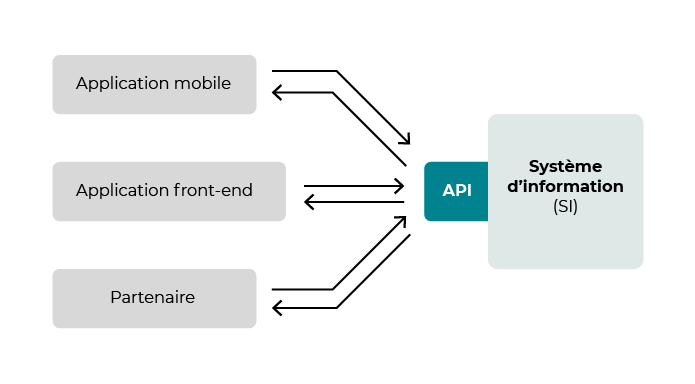
\includegraphics[width=10cm]{images/image01.png}
\end{center}

Une API peut être créée dès le début d’un projet, mais aussi être mise en place sur un projet existant pour le faire évoluer. C’est ce dernier que nous allons ensuite voir ensemble, en {\bf adaptant un projet Django existant pour lui intégrer une API avec {\color{monOrange}Django REST Framework}} (DRF).
\subsection{Découvrez le cas concret du cours}
Tout au long de ce cours, nous allons {\em mettre en place une {\color{monOrange}API}} sur un projet de boutique en ligne qui permet à des utilisateurs de consulter un catalogue de produits rangé par catégories, produits et articles. 

Nous permettrons ensuite aux {\color{monOrange}administrateurs de la plateforme de gérer la boutique} en ligne, en ajoutant de nouveaux produits à mettre en vente, et en masquant certains produits s’ils ne sont plus disponibles. Nous devrons alors sécuriser certains endpoints pour qu’ils ne soient pas accessibles publiquement.

Le code de l’application est disponible sur ce repository. À la fin de certains chapitres, des exercices seront proposés en partant d’une branche {\color{monOrange}Git}, et une solution sera proposée dans une autre branche.
\subsection{Installez et configurez {\color{monOrange}DRF}}
Django REST Framework est une librairie permettant la mise en place d’une API pour Django (vous pouvez regarder sa documentation sur le site officiel, en anglais). Basée sur le framework, elle propose la mise en place des endpoints d’une façon similaire à la mise en place des URL, Views et Forms de Django.
\subsubsection*{Pourquoi utilise-t-on cette librairie ?}
Écrire une API à la main est possible, on pourrait écrire nous-mêmes nos endpoints en nous basant sur les Views de Django, et retourner du JSON.

Mais c’est en réalité une quantité de travail phénoménale, et d’autres développeurs se sont déjà penchés sur le sujet pour simplifier grandement l’écriture d’API.

Dans ce chapitre, nous allons faire simple et :
\begin{itemize}
\item Mettre en place la librairie, en l’ajoutant aux dépendances de notre projet ;
\item Déclarer DRF parmi les applications du projet Django pour permettre son utilisation ;
\item Configurer une première URL fournie par DRF pour s’assurer du bon fonctionnement de la librairie.
\end{itemize}
En partant de la \href{https://github.com/OpenClassrooms-Student-Center/7192416_APIs_DRF}{branche main de notre projet},
\begin{center}
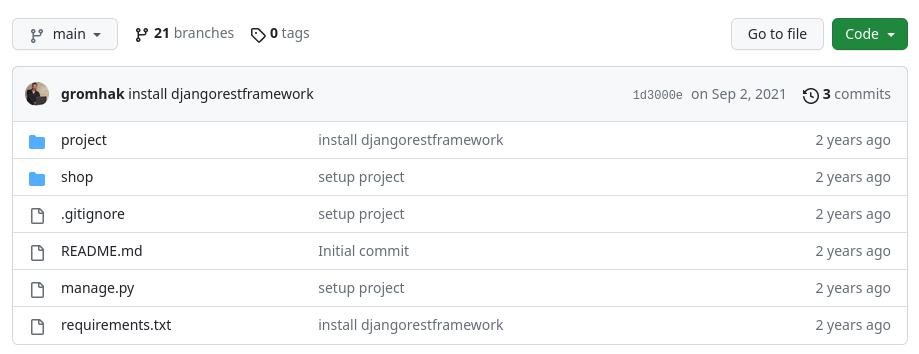
\includegraphics[width=10cm]{images/image02.png}
\end{center}
\begin{center}

\includegraphics[width=10cm]{images/image03.png}
\end{center}
 commençons par {\bf ajouter la dépendance à DRF} dans notre fichier {\color{monOrange}requirements.txt}  :
\begin{minted}[
mathescape,
framesep=2mm,
baselinestretch=1.2,
%fontsize=\footnotesize,
bgcolor=LightGray,
%linenos
]{latex}
djangorestframework==3.12.4
\end{minted}

Un petit coup d’ install  dans notre environnement virtuel :
\begin{minted}[
mathescape,
framesep=2mm,
baselinestretch=1.2,
%fontsize=\footnotesize,
bgcolor=LightGray,
%linenos
]{bash}
pip install -r requirements.txt
\end{minted}

Puis, déclarons DRF dans la liste des applications installées du fichier  settings.py  du projet Django :
\begin{minted}[
mathescape,
framesep=2mm,
baselinestretch=1.2,
%fontsize=\footnotesize,
bgcolor=LightGray,
%linenos
]{python}
INSTALLED_APPS = [
'rest_framework',
]
\end{minted}

Pour nous assurer que notre API est fonctionnelle, nous allons activer l’authentification fournie par DRF pour nous connecter. Éditons notre fichier  urls.py  :
\begin{minted}[
mathescape,
framesep=2mm,
baselinestretch=1.2,
%fontsize=\footnotesize,
bgcolor=LightGray,
%linenos
]{python}
urlpatterns = [
    path('api-auth/', include('rest_framework.urls'))
]
\end{minted}

Démarrons à présent notre serveur de développement et allons nous connecter sur notre API à présent en place :
\begin{minted}[
mathescape,
framesep=2mm,
baselinestretch=1.2,
%fontsize=\footnotesize,
bgcolor=LightGray,
%linenos
]{bash}
python manage.py runserver
\end{minted}

Nous devrions maintenant pouvoir nous rendre sur notre URL et nous connecter. Le projet contient une base de données SQLite qui contient déjà un compte administrateur dont voici les identifiants :
\begin{itemize}
\item Nom d’utilisateur : admin-oc
\item Mot de passe : password-oc
\end{itemize}

Le projet étant en local, nous pouvons nous connecter à l’URL

\url{http://127.0.0.1:8000/admin}.

Nous avons installé et configuré DRF !
\begin{center}
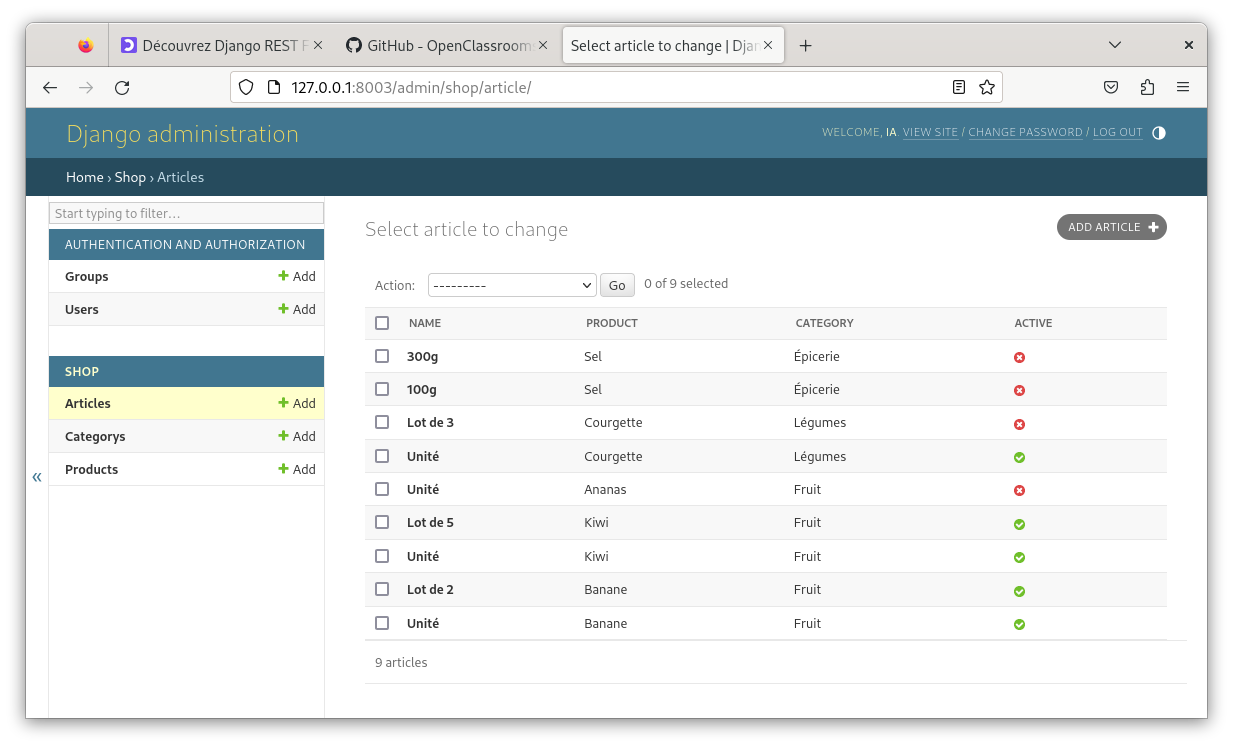
\includegraphics[width=15cm]{images/image04.png}
\end{center}
\subsubsection*{En résumé}
\begin{itemize}
\item Les API sont des interfaces permettant l’échange et le traitement d’informations entre un système d’information et toute autre application.
\item Un endpoint est une URL sur laquelle on peut effectuer des opérations en fonction de la méthode HTTP utilisée.
\item Django Rest Framework est une librairie permettant de mettre en place une API sur un projet Django.
\end{itemize}

{\em Maintenant, on est prêts pour la suite, et sans attendre on va mettre en place notre premier endpoint !}

\section{Gérez des données avec un endpoint}
\subsection{Créez un premier endpoint}
En avant, mettons en place ce premier {\color{monOrange}endpoint} en permettant à nos visiteurs d’accéder à la liste des catégories de nos produits. La toute première chose à faire lors de la réalisation d’un endpoint est de se demander {\bf quelles sont les informations importantes que nous souhaitons en tirer}.

Dans notre cas, pour afficher la liste des catégories, nous allons avoir besoin de leur nom, mais également de leur {\color{monOrange}identifiant}. L’identifiant sera utile aux clients (application front, mobile…) pour identifier de manière claire et unique les catégories s’ils ont des actions à faire dessus, comme afficher les produits qui constituent une catégorie.

DRF met à notre disposition des {\color{monOrange}serializers} qui permettent de transformer nos models Django en un autre format qui, lui, est exploitable par une API. Lorsque notre API sera consultée, le {\em serializer} va nous permettre de transformer notre objet en un JSON et, inversement, lorsque notre API va recevoir du JSON, elle sera capable de le transformer en un objet.

Pour le développeur qui les utilise, ils fonctionnent à la manière des formulaires proposés par Django. C'est-à-dire qu’ils sont paramétrés en précisant le model à utiliser et les champs de ce model à sérialiser.

\begin{theorem}
Pour rappel, un {\tt modelDjango} est une classe matérialisée dans la base de données, et qui permet donc l’utilisation de l’Object-Relational Mapping ({\color{monOrange}ORM}) de Django. Il sert à représenter et faire persister les données métier de notre système d’information. Dans notre cas, il s’agit des catégories, produits et articles mis en vente sur notre boutique.
\end{theorem}
Créons un fichier  {\tt serializers.py}  et {\em écrivons notre premier {\color{monOrange}serializer}}, que nous nommerons  {\tt CategorySerializer}  pour rester clair et précis. ;)

Il est nécessaire de définir sa classe  {\tt Meta}  et la liste des champs, exactement comme pour un formulaire. De plus, les noms des attributs sont identiques.
\begin{minted}[
mathescape,
framesep=2mm,
baselinestretch=1.2,
%fontsize=\footnotesize,
bgcolor=LightGray,
%linenos
]{python}
from rest_framework.serializers import ModelSerializer
from shop.models import Category
 
class CategorySerializer(ModelSerializer):
    class Meta:
        model = Category
        fields = ['id', 'name']

\end{minted}
Occupons-nous à présent de la {\color{monOrange}View}. {\bf DRF} nous propose une  {\color{monOrange}APIView}  qui a également un fonctionnement similaire aux  {\tt Views}  de Django.

Nous devons réécrire la méthode  {\color{monOrange}get}  qui réalisera les actions suivantes :
\begin{itemize}
\item Récupérer toutes les catégories en utilisant l’ORM de Django ;
\item Sérialiser les données à l’aide de notre serializer ;
\item Renvoyer une réponse qui contient les données sérialisées.
\end{itemize}
\begin{minted}[
mathescape,
framesep=2mm,
baselinestretch=1.2,
%fontsize=\footnotesize,
bgcolor=LightGray,
%linenos
]{python}
from rest_framework.views import APIView
from rest_framework.response import Response
from shop.models import Category
from shop.serializers import CategorySerializer
 
class CategoryAPIView(APIView):
    def get(self, *args, **kwargs):
        categories = Category.objects.all()
        serializer = CategorySerializer(categories, many=True)
        return Response(serializer.data)
\end{minted}
Le paramètre  {\color{monOrange}many}  permet de préciser au {\color{monOrange}Serializer} qu’il va devoir générer une liste d’éléments à partir de l’itérable (notre {\color{monOrange}queryset}) qui lui est transmis.

\subsubsection*{Et si je n’ai qu’un seul élément à sérialiser ?}
Dans ce cas, il n’est pas nécessaire de préciser le paramètre  {\color{monOrange}many}, et l’objet peut directement être donné au {\color{monOrange}Serializer} sans le mettre dans un {\em itérable}. Enfin, pour obtenir les données sérialisées, nous appelons la propriété  {\tt data}  de notre serializer. Ce sont ces données qui sont utilisées pour construire la réponse. Il ne reste plus qu’à créer l’{\color{monOrange}URL} correspondante et l’associer à notre {\color{monOrange}View} :
\begin{minted}[
mathescape,
framesep=2mm,
baselinestretch=1.2,
%fontsize=\footnotesize,
bgcolor=LightGray,
%linenos
]{python}
from django.contrib import admin
from django.urls import path, include
from shop.views import CategoryAPIView
 
urlpatterns = [
    path('admin/', admin.site.urls),
    path('api-auth/', include('rest_framework.urls')),
    path('api/category/', CategoryAPIView.as_view())
]
\end{minted}
Notre endpoint est maintenant accessible sur l’URL \url{http://127.0.0.1:8000/api/category/} . L’interface proposée par {\color{monOrange}DRF} nous permet de voir également le status code obtenu. Dans notre cas, 200, qui indique un succès. 
\begin{center}
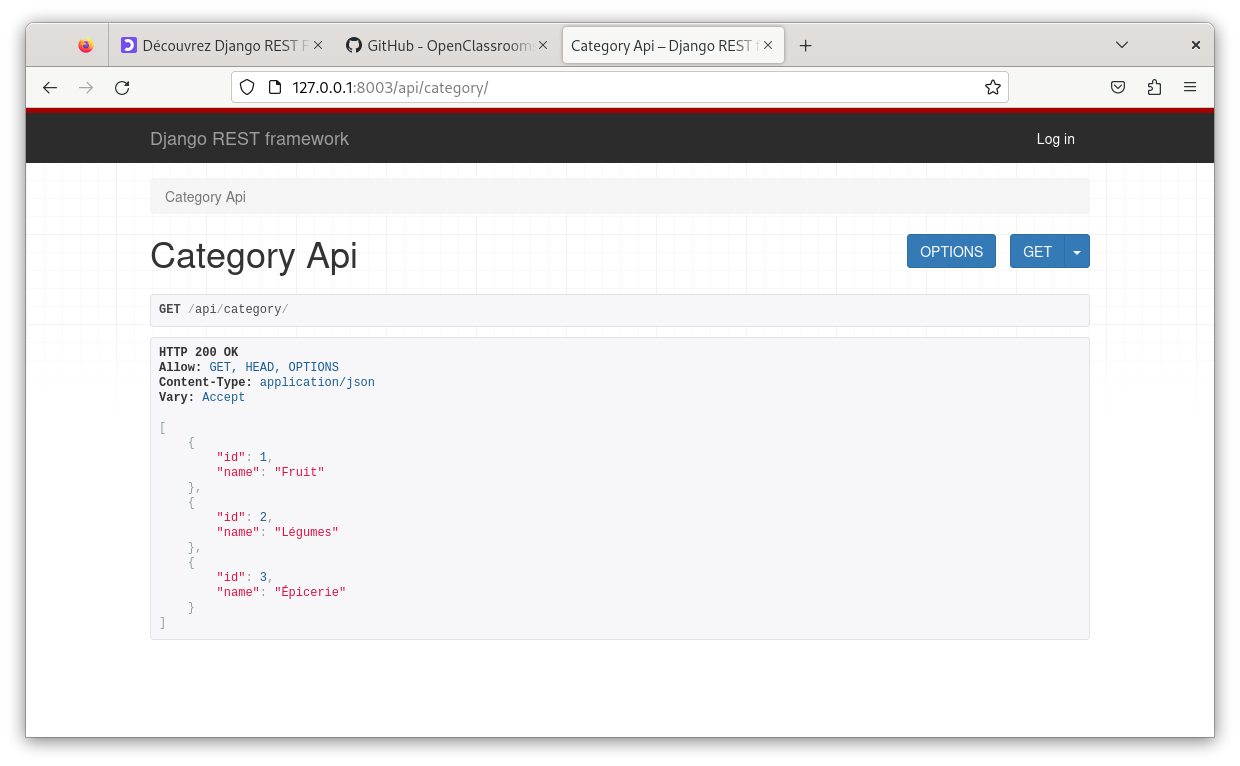
\includegraphics[width=15cm]{images/image05.png}
\end{center}

N’hésitez pas à jouer avec notre nouveau serializer, lui ajouter des champs, comme les dates de création et de modification. Tentez l’écriture pour les autres méthodes HTTP, l’expérimentation est un levier !

\subsection{Découvrez les méthodes d’un {\color{monOrange}endpoint}}
Seul {\color{monOrange}GET} est accessible sur notre endpoint, car nous n’avons redéfini que la méthode  {\color{monOrange}get}  dans la {\color{monOrange}View}. Ne pas réécrire de méthodes permet de ne pas les rendre accessibles. Nous pourrions réécrire également les méthodes  {\color{monOrange}post,  patch}  et  {\color{monOrange}delete}. 

\subsubsection{{\tt GET} et {\tt POST} servent avec Django à créer de nouvelles entités au travers de formulaires, mais {\tt PATCH} et {\tt DELETE} servent à quoi ?}
Reprenons-les une par une pour voir réellement à quoi servent ces méthodes HTTP dans le cadre d’une API, et les différences avec un site Internet classique :
\begin{itemize}
\item {\color{monOrange}GET} : Permet la lecture d'informations.
Un peu comme un site Internet classique, les appels en GET renvoient des données qui sont généralement du HTML qui est lu et rendu dans le navigateur. Dans le cas d’une API, il s’agit de JSON.
\item {\color{monOrange}POST} : Permet la création d’entités.
Alors que sur un site les appels en POST peuvent être utilisés pour modifier une entité, dans le cas d’une API, les POST permettent la création.
\item {\color{monOrange}PATCH} : Permet la modification d’une entité.
PATCH permet la modification de tout ou partie des valeurs des attributs d’une entité pour une API, alors que pour un site classique, nous utilisons un formulaire et un POST.
\item {\color{monOrange}DELETE} : Permet la suppression d’une entité.
DELETE permet la suppression d’une entité pour une API, alors que pour un site classique, nous utilisons un formulaire et généralement un POST.
\item {\color{monOrange}PUT} : Permet également la modification d’une entité.
Il est peu utilisé en dehors de l’interface de DRF, que nous verrons ensuite. Pour un site classique, l’action de modification entière d’une entité passe également par un POST au travers d’un formulaire.
\end{itemize}

Pas de panique, tout n’est pas à retenir tout de suite. Durant ce cours, nous allons aborder chacune de ces méthodes dans divers cas pratiques.

Ce qui est important à retenir est que chaque méthode correspond à une action du CRUD (Create, Read, Update, Delete), et c’est cela qui va nous permettre d’agir directement sur nos models.

\subsubsection*{Exercice}
Je vous propose de prendre la main et de mettre en place un nouvel endpoint qui va permettre de lister tous les produits de notre boutique en ligne. Utilisons l’URL suivante : \url{http://127.0.0.1:8000/api/product/}. Cet endpoint doit retourner les informations suivantes des produits :
\begin{itemize}
\item Son identifiant  {\tt id}.
\item Sa date de création  {\tt date\_created}.
\item Sa date de modification  {\tt date\_updated}.
\item Son nom  {\tt name}.
\item L’identifiant de la catégorie à laquelle il appartient  {\tt category}.
\end{itemize}
Pour réaliser cela, vous pouvez partir de la branche \href{https://github.com/OpenClassrooms-Student-Center/7192416\_APIs\_DRF/tree/P1C3\_exercice}{P1C3\_exercice}. Elle contient déjà ce que nous venons de faire ensemble. Une solution est proposée sur la branche \href{https://github.com/OpenClassrooms-Student-Center/7192416\_APIs\_DRF/tree/P1C3\_solution}{P1C3\_solution}.

\subsubsection*{En résumé}
\begin{enumerate}
\item Le fonctionnement des serializers proposé par DRF est similaire à celui des formulaires de Django.
\item Les serializers permettent de faire une représentation de nos models en JSON.
\item Les méthodes HTTP utilisables sont la représentation du CRUD (Create, Read, Update, Delete).
\item DRF nous propose une interface web qui permet de visualiser notre API.
\end{enumerate}
N’hésitez pas à modifier les données que retournent le serializer. Imaginez le but de l’endpoint que vous êtes en train de mettre en place pour déterminer quelles sont les données les plus pertinentes à retourner.
\section{Rendez les Views plus génériques avec un ModelViewset}
\section{Mettez en place un {\color{monOrange}router}}
Plutôt que de créer nos URL et de redéfinir nos méthodes une à une, DRF propose des classes héritables pour nos vues, qui sont les {\color{monOrange}ModelViewsets}. Elles permettent la mise en place rapide de toutes les actions du CRUD pour un model donné. Utiliser un ModelViewset nécessite d’utiliser une autre façon de définir nos URL. Cela se fait au travers d’un {\color{monOrange}router}.
\subsection*{Un router, c’est quoi ?}
Un router permet de définir automatiquement toutes les URL accessibles pour un endpoint donné. Il va à la fois permettre de définir :
\begin{itemize}
\item L’URL  {\tt /api/category/}, qui permet de réaliser des actions globales qui ne concernent pas directement une entité précise, comme la récupération de la liste des entités ou la création d’une nouvelle.
\item L’URL  {\tt /api/category/<pk>/}, qui en acceptant un paramètre correspondant à l’identifiant d’une entité, va permettre de réaliser des actions sur celle-ci, comme obtenir des informations, la modifier ou la supprimer.
\end{itemize}
{\em Mettons en place notre {\color{monOrange}router}} dans notre fichier {\tt urls.py}  et supprimons notre ancien {\color{monOrange}endpoint}: 
\begin{minted}[
mathescape,
framesep=2mm,
baselinestretch=1.2,
%fontsize=\footnotesize,
bgcolor=LightGray,
%linenos
]{python}
from django.contrib import admin
from django.urls import path, include
from rest_framework import routers
from shop.views import CategoryViewset
 
# Ici nous créons notre routeur
router = routers.SimpleRouter()
# Puis lui déclarons une url basée sur le mot clé ‘category’ et notre view
# afin que l’url générée soit celle que nous souhaitons ‘/api/category/’
router.register('category', CategoryViewset, basename='category')
 
urlpatterns = [
    path('admin/', admin.site.urls),
    path('api-auth/', include('rest_framework.urls')),
    path('api/', include(router.urls))  # Il faut bien penser à ajouter les 
    # urls du router dans la liste des urls disponibles.
]
\end{minted}
Le router se définit en amont de la définition de  {\tt urlpatterns}. Les URL sont incluses avec un  {\tt include}  au travers de la propriété  {\tt router.urls}. Notons également qu’il n’est plus nécessaire d'appeler  {\tt .as\_view()}, le router le fait pour nous lorsqu’il génère les URL.

\begin{theorem}
Le paramètre {\tt basename}  permet de retrouver l’URL complète avec la fonction {\tt redirect}, comme le propose Django. Cela sera utile lors de l’écriture des tests que nous aborderons ensuite.
\end{theorem}

\subsection{Transformez une ApiView en ModelViewset}
À présent, nous devons transformer notre  {\color{monOrange}ApiView}  en un  {\color{monOrange}ModelViewset} pour que notre vue puisse être connectée à notre routeur. Un {\color{monOrange}ModelViewset}  est comparable à une super vue Django qui regroupe à la fois {\color{monOrange}CreateView, UpdateView, DeleteView, ListView}  et {\color{monOrange}DetailView}. Il faut impérativement lui {\em définir deux attributs de classe }:
\begin{enumerate}
\item {\tt serializer\_class}  qui va déterminer le {\tt serializer} à utiliser ;
\item {\tt queryset}, ou réécrire la méthode {\tt get\_queryset}  qui doit retourner un {\color{monOrange}Queryset} des éléments à retourner.
\end{enumerate}
\begin{theorem}
Redéfinir seulement l’attribut de classe {\tt queryset}  permet principalement de faire des tests rapides. À l’usage, redéfinir {\tt get\_queryset}  est souvent la solution à adopter car elle permet d’être plus fin sur les éléments à retourner.
\end{theorem}
\begin{minted}[
mathescape,
framesep=2mm,
baselinestretch=1.2,
%fontsize=\footnotesize,
bgcolor=LightGray,
%linenos
]{python}
from rest_framework.viewsets import ModelViewSet
from shop.models import Category
from shop.serializers import CategorySerializer
 
class CategoryViewset(ModelViewSet):
 
    serializer_class = CategorySerializer
 
    def get_queryset(self):
        return Category.objects.all()
\end{minted}
Nous pouvons dès à présent retester notre API à l’adresse \url{http://127.0.0.1:8000/api/category/}.
Le résultat est identique à ce que nous avions précédemment. La différence étant qu’il nous est maintenant possible de réaliser directement les autres opérations du {\color{monOrange}CRUD}. Le formulaire en bas de page vous invite directement à réaliser un {\color{monOrange}POST} pour créer une nouvelle catégorie.
\begin{center}
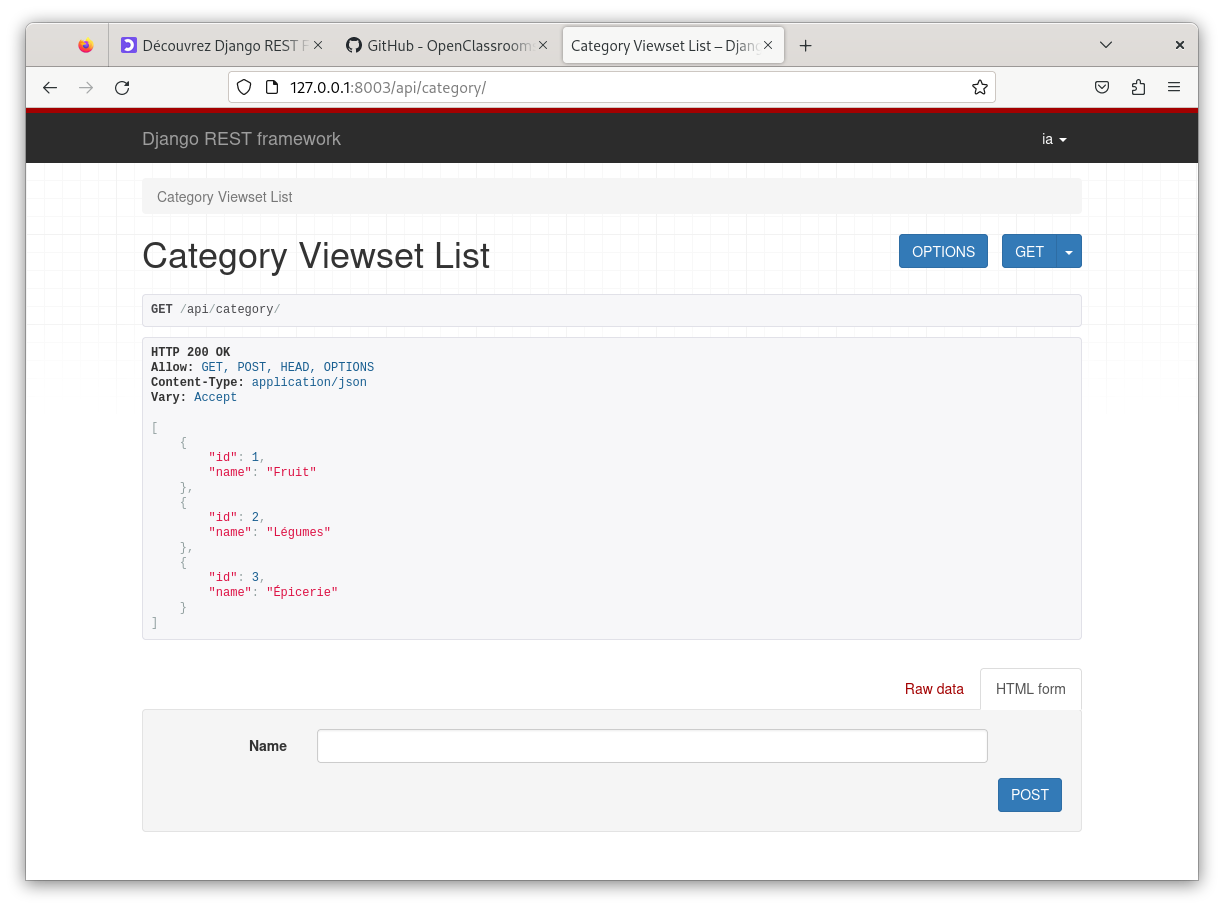
\includegraphics[width=10cm]{images/image06.png}
\end{center}
Le détail d’une catégorie est également visible en ajoutant son identifiant dans l’URL, par exemple \url{http://127.0.0.1:8000/api/category/1/}. La page vous propose alors de réaliser les actions {\color{monOrange}PUT, PATCH} (dans l’onglet « Raw data ») et {\color{monOrange}DELETE} sur l’entité consultée.
\begin{center}
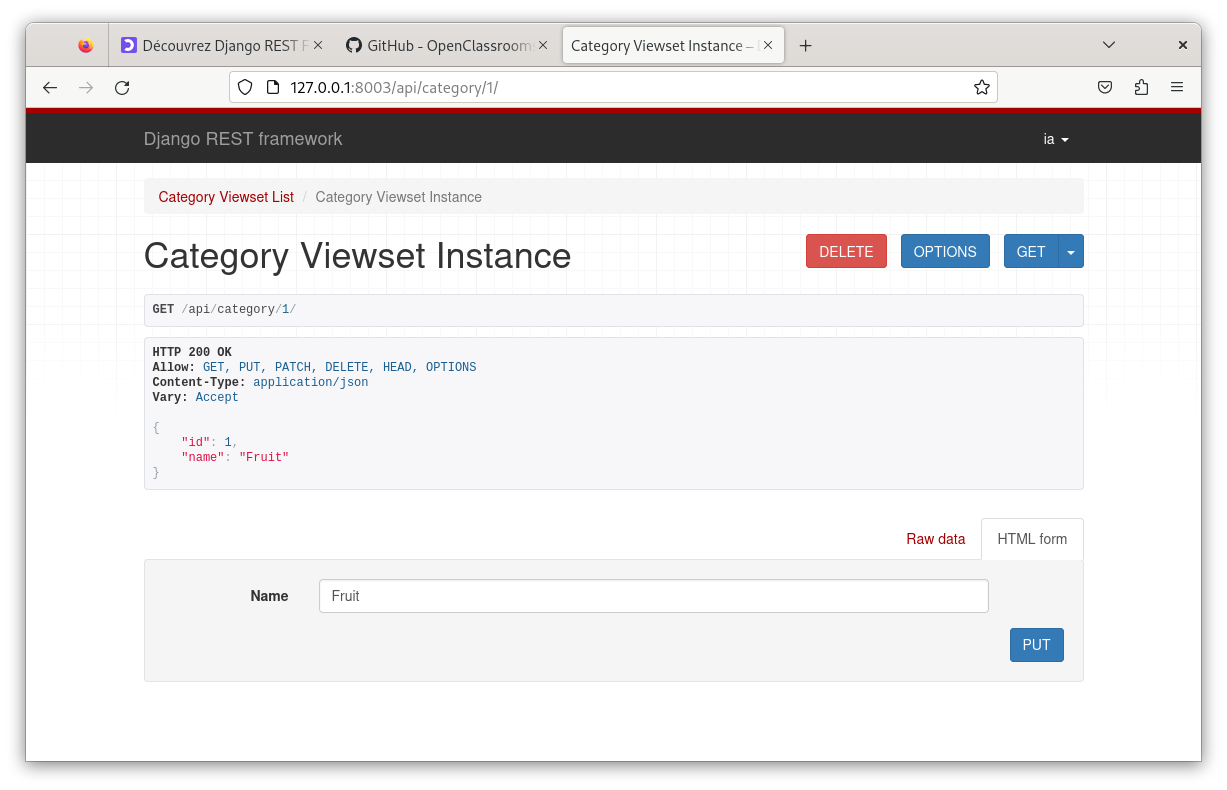
\includegraphics[width=10cm]{images/image07.png}
\end{center}
\subsection{Ne permettez que la lecture}
Vous l’aurez sûrement remarqué, nous pouvons créer de nouvelles catégories ; dans la pratique, permettre la création, la modification et la suppression sur un endpoint public comme le nôtre n’est pas conseillé. Nous allons donc faire en sorte que notre endpoint {\em ne permette que la lecture}, car son but est d’afficher à nos utilisateurs la liste des catégories disponibles sur la boutique. Pour cela, DRF nous propose un autre type de {\color{monOrange}ModelViewset}. Il s’agit du {\color{monOrange}ReadOnlyModelViewset}  qui, comme son nom l’indique, ne permet que la lecture.

Modifions notre vue pour limiter les opérations disponibles. Nous allons faire étendre la vue CategoryViewset  avec le {\tt viewset} {\color{monOrange}ReadOnlyModelViewset}   au lieu du {\color{monOrange}ModelViewset}  actuel.
\begin{minted}[
mathescape,
framesep=2mm,
baselinestretch=1.2,
%fontsize=\footnotesize,
bgcolor=LightGray,
%linenos
]{python}
from rest_framework.viewsets import ReadOnlyModelViewSet
from shop.models import Category
from shop.serializers import CategorySerializer
 
class CategoryViewset(ReadOnlyModelViewSet):
    serializer_class = CategorySerializer
    def get_queryset(self):
        return Category.objects.all()
\end{minted}
Si nous consultons à présent notre API, nous pouvons constater que toutes les options autres que la lecture ne sont plus permises.
\begin{center}
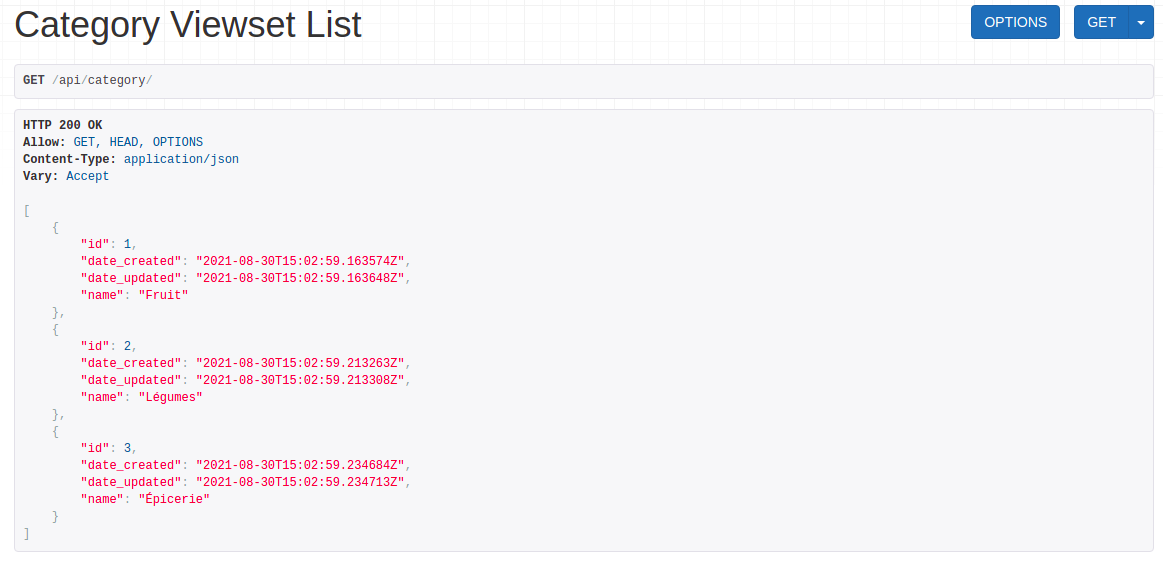
\includegraphics[width=10cm]{images/image08.png}
\end{center}
\begin{theorem}
Il est également possible d’utiliser l’attribut   {\tt read\_only\_fields}  sur le serializer pour préciser les champs en lecture seule. Mais cela n'empêchera pas les actions de création, modification et suppression.
\end{theorem}
\subsubsection*{Exercice}
Notre endpoint de consultation de produits ne doit également permettre que la lecture. Entraînez-vous dans l’utilisation des Viewsets  pour passer cet endpoint en « lecture seule ».
\begin{itemize}
\item Pour réaliser cela, vous pouvez partir de la branche \href{https://github.com/OpenClassrooms-Student-Center/7192416\_APIs\_DRF/tree/P1C4\_exercice}{P1C4\_exercice}. Elle contient déjà ce que nous venons de faire ensemble.
\item Une solution est proposée sur la branche \href{https://github.com/OpenClassrooms-Student-Center/7192416\_APIs\_DRF/tree/P1C4_solution}{P1C4\_solution}.
\end{itemize}
\subsubsection*{En résumé}
\begin{enumerate}
\item Un router permet de définir en une seule fois toutes les opérations du CRUD sur un endpoint.
\item Utiliser un  {\tt ModelViewset}  impose d’utiliser un router pour définir ses URL.
\item Lors de l’utilisation d’un {\tt ModelViewset}, il faut définir :
\begin{enumerate}
\item le serializer à utiliser avec l’attribut de classe {\tt serializer\_class}  ;
\item le jeu de données qui sera retourné en réécrivant la méthode {\tt get\_queryset}.
\end{enumerate}
\item {\tt ReadOnlyModelViewset}  permet de limiter les accès à la lecture seule.
\end{enumerate}
{\em Les Viewsets sont très souvent les vues à privilégier, nous allons dès maintenant voir comment les personnaliser et les adapter avec plus de précision à nos besoins. Suivez-moi au prochain chapitre !}

\section{Filtrez les résultats d’un endpoint}
\subsection{Appliquez un filtre sur les données retournées}
Lorsque nos utilisateurs naviguent sur notre boutique, il se peut qu’ils souhaitent récupérer les produits d’une catégorie grâce à un appel fait à notre API. Sauf que pour le moment, notre endpoint de produits ne permet pas de {\em filtrer par catégorie}. Pour réaliser cela, nous allons accepter un paramètre dans l’URL qui sera l’identifiant de la catégorie, pour ne renvoyer que les produits correspondants. Le paramètre sera nommé {\tt category\_id}, ce qui donnera une URL sous le format
\begin{center}
\url{http://127.0.0.1:8000/api/product/?category_id=1}.
\end{center}
Éditons notre classe {\tt ProductViewset}  pour qu’elle applique un nouveau filtre si le paramètre est présent. Profitons-en pour également appliquer le filtre sur les produits actifs :
\begin{minted}[
mathescape,
framesep=2mm,
baselinestretch=1.2,
%fontsize=\footnotesize,
bgcolor=LightGray,
%linenos
]{python}
class ProductViewset(ReadOnlyModelViewSet):
    serializer_class = ProductSerializer
    def get_queryset(self):
    # Nous récupérons tous les produits dans une variable nommée queryset
        queryset = Product.objects.filter(active=True)
        # Vérifions la présence du paramètre ‘category_id’ dans l’url et si oui alors appliquons notre filtre
        category_id = self.request.GET.get('category_id')
        if category_id is not None:
            queryset = queryset.filter(category_id=category_id)
        return queryset
\end{minted}

À présent, nous pouvons constater que le filtre est bien appliqué si nous consultons la liste des produits de la catégorie 1 avec l’URL 

\begin{center}
\url{http://127.0.0.1:8000/api/product/?category_id=1}.
\end{center}
\begin{center}
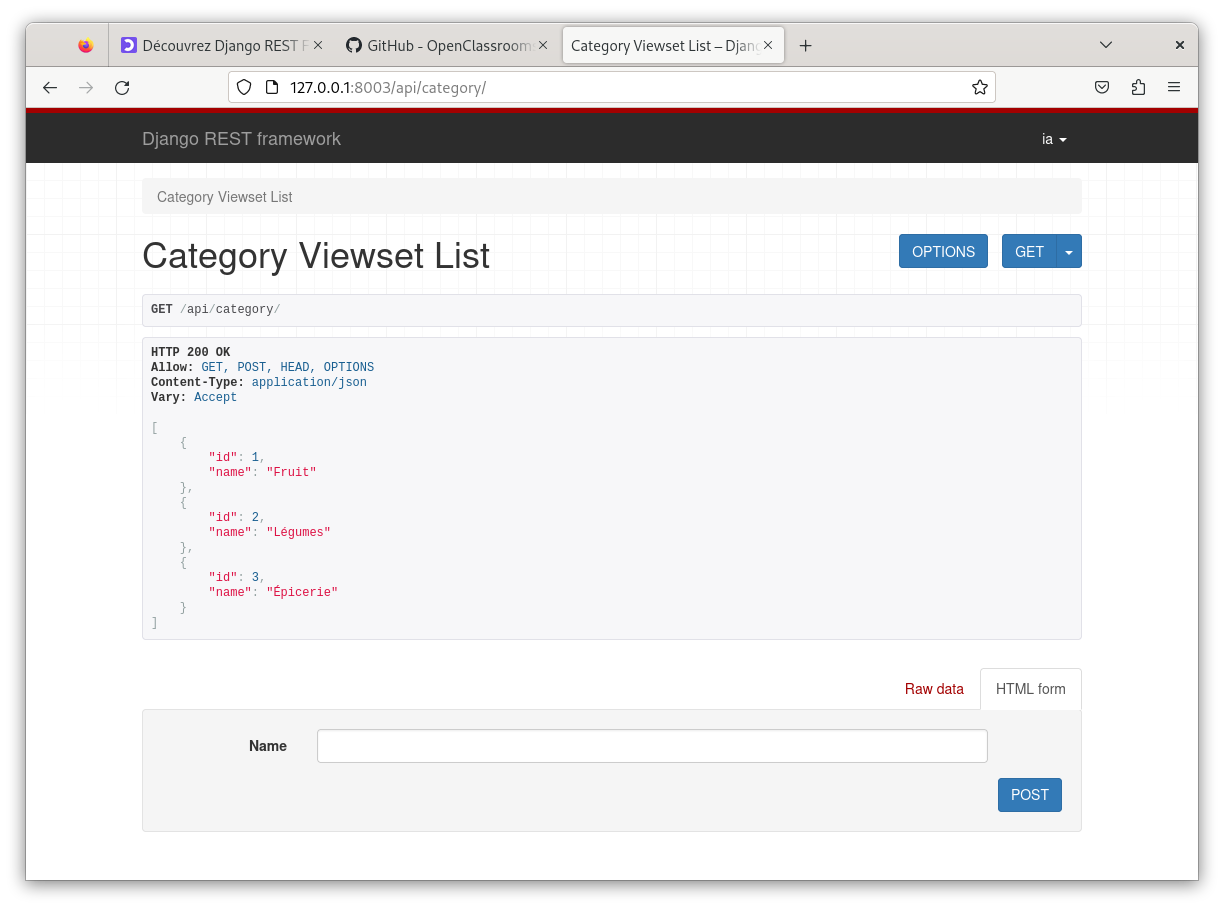
\includegraphics[width=10cm]{images/image09.png}
\end{center}
Et si nous demandons une catégorie qui n'existe pas, alors une liste de produits vide est retournée sans faire planter notre application :
\begin{center}
\url{http://127.0.0.1:8000/api/product/?category_id=7777777}.
\end{center}
\begin{center}
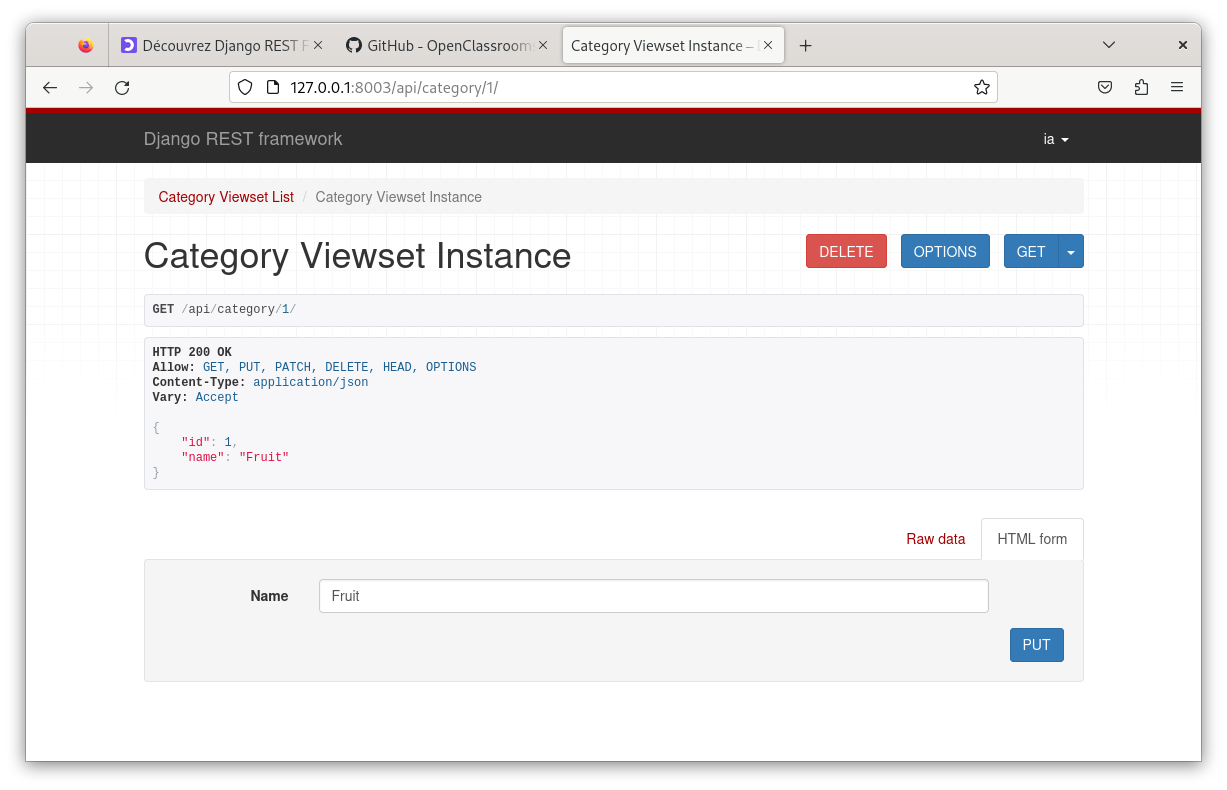
\includegraphics[width=10cm]{images/image10.png}
\end{center}

Ainsi, les paramètres d’URL peuvent servir à appliquer {\em toutes sortes de filtres sur les données retournées}. N’hésitez pas à jouer avec, en permettant par exemple de forcer l’affichage des produits inactifs.
\begin{theorem}
Nous aurions pu améliorer encore notre endpoint, en lui ajoutant un paramètre permettant d’inclure les catégories non disponibles, par exemple. N’hésitez pas à les utiliser, ils sont souvent une solution qui évite la création d’un nouvel endpoint.
\end{theorem}

\subsubsection*{Exercice}
À votre tour ! Pour parfaire notre boutique, nous souhaitons mettre en place un endpoint de récupération des articles sur l’URL http://127.0.0.1:8000/api/article/. Il ne doit retourner que les articles actifs, et permettre de filtrer les articles retournés sur une catégorie avec un paramètre {\tt product\_id}.
Cet endpoint doit retourner les informations suivantes :
\begin{itemize}
\item L’identifiant de l’article ;
\item La date de création et de modification de l’article ;
\item Le nom de l’article ;
\item Le prix de l’article ;
\item L’identifiant du produit auquel appartient l’article.
\end{itemize}
Pour réaliser cela, vous pouvez partir de la branche \href{https://github.com/OpenClassrooms-Student-Center/7192416\_APIs\_DRF/tree/P1C5\_exercice}{P1C5\_exercice}. Elle contient déjà ce que nous venons de faire ensemble. Une solution est proposée sur la branche \href{https://github.com/OpenClassrooms-Student-Center/7192416\_APIs\_DRF/tree/P1C5\_solution}{P1C5\_solution}.

\subsubsection*{En résumé}
\begin{enumerate}
\item Redéfinir la méthode {\tt get\_queryset}  permet de définir les entités à prendre en compte dans l'endpoint.
\item Il est possible d’utiliser des paramètres d’URL pour apporter des précisions sur l’action à réaliser (comme filtrer sur un critère particulier).
\end{enumerate}

{\em C’est maintenant l’heure d’écrire les premiers tests pour notre API ! Rendez-vous au prochain chapitre.}

\section{Écrivez des tests pour votre API}
\subsection{Découvrez le TestCase de DRF}
Les tests sont un élément important de tout projet de développement. Ils permettent de garantir la pérennité du projet, sa maintenance, et surtout de déployer la conscience plus tranquille.

Une nouvelle classe de test {\color{monOrange}APITestCase}  est fournie par DRF. Elle est faite pour fonctionner de la même façon que la classe {\color{monOrange}TestCase}. Sa principale différence étant d’utiliser un client qui permet une utilisation plus simple des appels. Il est donc recommandé de l’utiliser pour ne pas avoir à définir plusieurs paramètres pour réaliser nos appels lors des tests.

\subsection{Écrivez des tests avec APITestCase}
Créons notre fichier de test dans l’application {\tt shop}  et mettons en place un test qui {\em vérifie l’endpoint de récupération des catégories actives}. Nous allons pour cela :
\begin{itemize}
\item Créer deux catégories dont une inactive ;
\item Réaliser notre appel ;
\item Vérifier que le status code de la réponse est bien un succès : 200 ; 
\item Nous assurer que le contenu de la réponse est bien celui attendu, et qu'il ne comprend pas la catégorie désactivée.
\end{itemize}
Nous écrirons aussi un test qui s’assurera que la création d’une catégorie n’est pas possible, et tombe bien en erreur.
\begin{theorem}
Il est très facile d’oublier d’écrire des tests pour les cas positifs en erreur. Notre API étant pour le moment publique, il est important de tester qu’un utilisateur ne puisse pas créer de nouvelles catégories.
\end{theorem}
Créons d'abord un fichier  {\tt tests.py}  pour nos tests. Puis, c’est parti pour nos deux tests :
\begin{minted}[
mathescape,
framesep=2mm,
baselinestretch=1.2,
fontsize=\footnotesize,
bgcolor=LightGray,
%linenos
]{python}
from django.urls import reverse_lazy
from rest_framework.test import APITestCase

from shop.models import Category

class TestCategory(APITestCase):
    # Nous stockons l’url de l'endpoint dans un attribut de classe pour pouvoir
    # l’utiliser plus facilement dans chacun de nos tests
    url = reverse_lazy('category-list')

    def format_datetime(self, value):
        # Cette méthode est un helper permettant de formater une date en chaine de caractères 
        # sous le même format que celui de l’api
        return value.strftime("%Y-%m-%dT%H:%M:%S.%fZ")

    def test_list(self):
        # Créons deux catégories dont une seule est active
        category = Category.objects.create(name='Fruits', active=True)
        Category.objects.create(name='Légumes', active=False)

        # On réalise l’appel en GET en utilisant le client de la classe de test
        response = self.client.get(self.url)
        # Nous vérifions que le status code est bien 200
        # et que les valeurs retournées sont bien celles attendues
        self.assertEqual(response.status_code, 200)
        excepted = [
            {
                'id': category.pk,
                'name': category.name,
                'date_created': self.format_datetime(category.date_created),
                'date_updated': self.format_datetime(category.date_updated),
            }
        ]
        self.assertEqual(excepted, response.json())

    def test_create(self):
        # Nous vérifions qu’aucune catégorie n'existe avant de tenter d’en créer une
        self.assertFalse(Category.objects.exists())
        response = self.client.post(self.url, data={'name': 'Nouvelle catégorie'})
        # Vérifions que le status code est bien en erreur et nous empêche de créer une catégorie
        self.assertEqual(response.status_code, 405)
        # Enfin, vérifions qu'aucune nouvelle catégorie n’a été créée malgré le status code 405
        self.assertFalse(Category.objects.exists())
\end{minted}

\begin{theorem}
Lors d’un développement, il vaut mieux prendre le temps d’écrire les tests au fil de l’eau, ce qui est moins décourageant que de les écrire tous à la fin. Parfois il peut aussi être intéressant de commencer par écrire le test avant de développer la fonctionnalité.
\end{theorem}
\subsubsection*{Exercice}
Écrivez vous aussi des tests pour l’endpoint de produits. Il peut également être intéressant de créer une classe de test pour notre projet, contenant notre méthode d’aide au formatage de date, qui sera étendu par nos classes de tests.
\begin{itemize}
\item Mettez en place une classe {\tt ShopAPITestCase}.
\item Refactorisez  {\tt TestCategory}  pour qu’elle étende notre nouvelle classe  {\tt ShopAPITestCase}.
\item Écrivez la classe de test  {\tt TestProduct}  qui va tester :
\begin{itemize}
\item l’endpoint de liste et de détail d’un produit ;
\item que le filtre sur la liste fonctionne correctement ;
\item qu’il n’est pas possible de créer, modifier et supprimer un produit.
\end{itemize}
\end{itemize}
Pour réaliser cela, vous pouvez partir de la branche \href{https://github.com/OpenClassrooms-Student-Center/7192416\_APIs\_DRF/tree/P1C6\_exercice}{P1C6\_exercice}. Elle contient déjà ce que nous venons de faire ensemble. Une solution est proposée sur la branche \href{https://github.com/OpenClassrooms-Student-Center/7192416\_APIs\_DRF/tree/P1C6\_solution}{P1C6\_solution}.

\subsubsection*{En résumé}
\begin{enumerate}
\item DRF met à disposition une classe de tests qu’il faut utiliser pour tester une API.
\item Il est important de tester le status code de retour ainsi que le contenu de la réponse.
\item Ne pas oublier de tester les cas d’erreur.
\item Les tests ne sont pas la partie la plus intéressante à écrire, mais ils garantissent la stabilité d’un projet dans le temps.
\end{enumerate}
{\em Nous voilà avec une API DRF simple et validée par nos premiers tests ! Avant de passer à l’étape suivante, validez vos acquis dans le quiz de la partie 1 – je vous attends dans la partie 2 !}




\end{document}











    \chapter{Rendez vos endpoints plus performants}
    \documentclass[a4paper]{article}
 
% - taille de la fonte    : 10pt, 11pt, 12pt
% - recto ou recto-verso    : oneside, twoside
 
% Chargement d'extensions
%\usepackage[latin1]{inputenc}    
\usepackage[francais]{babel}    
\AtBeginDocument{\def\labelitemi{$\bullet$}}

\usepackage{amsmath}
\makeatletter
%%%%%%%%%%%%%%%%%%% debut fichier boiboites.sty %%%%%%%%%%%%%%%%%%%%%%
\RequirePackage{xkeyval}
\RequirePackage{tikz}
\RequirePackage{amssymb}

\define@key{boxedtheorem}{titlecolor}{\def\titlecolor{#1}}
\define@key{boxedtheorem}{titlebackground}{\def\titlebackground{#1}}
\define@key{boxedtheorem}{background}{\def\background{#1}}
\define@key{boxedtheorem}{titleboxcolor}{\def\titleboxcolor{#1}}
\define@key{boxedtheorem}{boxcolor}{\def\boxcolor{#1}}
\define@key{boxedtheorem}{thcounter}{\def\thcounter{#1}}
\define@key{boxedtheorem}{size}{\def\size{#1}}
\presetkeys{boxedtheorem}{titlecolor = black, titlebackground = white, background = white,%
                         titleboxcolor = black, boxcolor = black, thcounter=, size = .9\textwidth}{}

\newcommand{\couleurs}[1][]{%
    \setkeys{boxedtheorem}{#1}
    \tikzstyle{fancytitle} =[draw=\titleboxcolor, rounded corners, fill=\titlebackground,
                            text= \titlecolor]
    \tikzstyle{mybox} = [draw=\boxcolor, fill=\background, very thick,
                        rectangle, rounded corners, inner sep=10pt, inner ysep=20pt]
}


%Commande generique pour faire un joli encadre
\newsavebox{\boiboite}
\newcommand{\titre}{Titre}
\newenvironment{boite}[2][]%
    {%
    \renewcommand{\titre}{#2}
    \couleurs[#1]
    \begin{lrbox}{\boiboite}%
     \begin{minipage}[!h]{\size}
    }%
    {%
     \end{minipage}
    \end{lrbox}
    \begin{center}
    \begin{tikzpicture}
    \node [mybox] (box){\usebox{\boiboite}};
    \node[fancytitle, right=10pt] at (box.north west) {\titre};
    \end{tikzpicture}
    \end{center}
    }

\newcommand{\newboxedtheorem}[4][]{%
    \couleurs[#1]
    \@ifnotempty{#4}{%
      \@ifundefined{the#4}{\@ifundefined{\thcounter}{\newcounter{#4}}{%
      \newcounter{#4}[\thcounter ] } } { }%
    }
    \newenvironment{#2}[1][]{%
    \@ifnotempty{#4}{\refstepcounter{#4}}
    \begin{boite}[#1]{\textbf{#3\@ifnotempty{#4}{ \csname the#4\endcsname}}\@ifnotempty{##1}{
    (##1)}}
    }%
    {%
    \end{boite}
    }
}
%%%%%%%%%%%%%%%%%%%% end fichier boiboites.sty %%%%%%%%%%%%%%%%%%%%%%
\makeatother
\newboxedtheorem{theorem}{}{theorem}
%%%%%%%%%% hypertext

\usepackage{hyperref}
\hypersetup{
    colorlinks=true,
    linkcolor=blue,
    filecolor=magenta,      
    urlcolor=cyan,
    pdftitle={Overleaf Example},
    pdfpagemode=FullScreen,
    }

\urlstyle{same}

%%%%%%%%%%%%%%%%%%%%%%%%%%%
\usepackage{amsthm}
%\usepackage{amsmath}
\usepackage{amssymb}
\usepackage{mathrsfs}
\usepackage{graphicx}
\usepackage{geometry}
\usepackage{stmaryrd}
\usepackage{tikz}
\usetikzlibrary{patterns}

\usepackage[cache=false]{minted}
\usepackage{xcolor}
%\setbeamercolor{background canvas}{bg=lightgray}
\definecolor{LightGray}{gray}{0.9}
\definecolor{monOrange}{rgb}{0.97,0.35,0.04}

% Informations le titre, le(s) auteur(s), la date
\title{Rendez vos endpoints plus performants}
\author{Ibrahim ALAME}
\date{\today}
\includeonly{ introduction.tex} 
\begin{document}
 
\maketitle
 %Mettez en place une API simple avec Django REST Framework
\section{Minimisez les appels de votre API grâce aux serializers}
\subsection{Retournez plus d'informations}
En l’état, les clients (application front, mobile, etc.) de notre API doivent réaliser {\em plusieurs appels} pour obtenir la liste des catégories et la liste des produits qui composent chacune d’entre elles.
\begin{center}
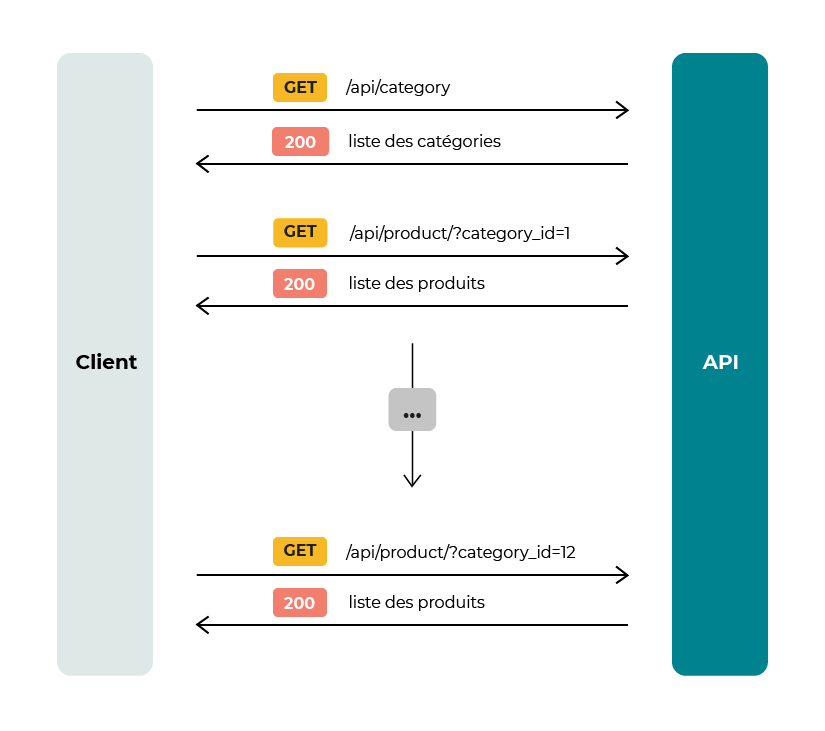
\includegraphics[width=12cm]{images/image11.png}
\end{center}
Donc autant d’appels qu’il y a de catégories sont nécessaires, ce qui n’est pas très optimal. Pour résoudre cette problématique, il est possible d’{\em imbriquer des serializers}, afin que le serializer des catégories renvoie directement la liste des produits qui composent la catégorie consultée. Et c’est ce que nous allons voir tout de suite ensemble.
\begin{theorem}
Attention tout de même à ne pas imbriquer trop de serializers car beaucoup d’appels en base de données peuvent être faits, à moins d’optimiser ces appels à l’aide de {\tt prefetch\_related}  et de {\tt select\_related} . Certains calculs de valeurs d’attributs peuvent aussi être coûteux, il faut donc utiliser l’imbrication avec parcimonie, selon les cas qui se présentent à nous.
\end{theorem}
\subsection{Imbriquez les serializers}
Nous allons faire en sorte que notre endpoint de catégorie renvoie également la liste des produits qui le composent. Pour cela, {\em éditons notre serializer de catégorie} en ajoutant dans la liste des fields le {\tt related\_name}  vers les produits définis dans notre model :
\begin{minted}[
mathescape,
framesep=2mm,
baselinestretch=1.2,
%fontsize=\footnotesize,
bgcolor=LightGray,
%linenos
]{python}
class CategorySerializer(ModelSerializer):
 
class Meta:
model = Category
        fields = ['id', 'date_created', 'date_updated', 'name', 'products']
\end{minted}
\begin{theorem}
Lorsque nous ajoutons un {\tt related\_name}  dans un serializer, DRF va ajouter la liste des identifiants distants dans un attribut portant le même nom que le {\tt related\_name}.
\end{theorem}

\begin{center}
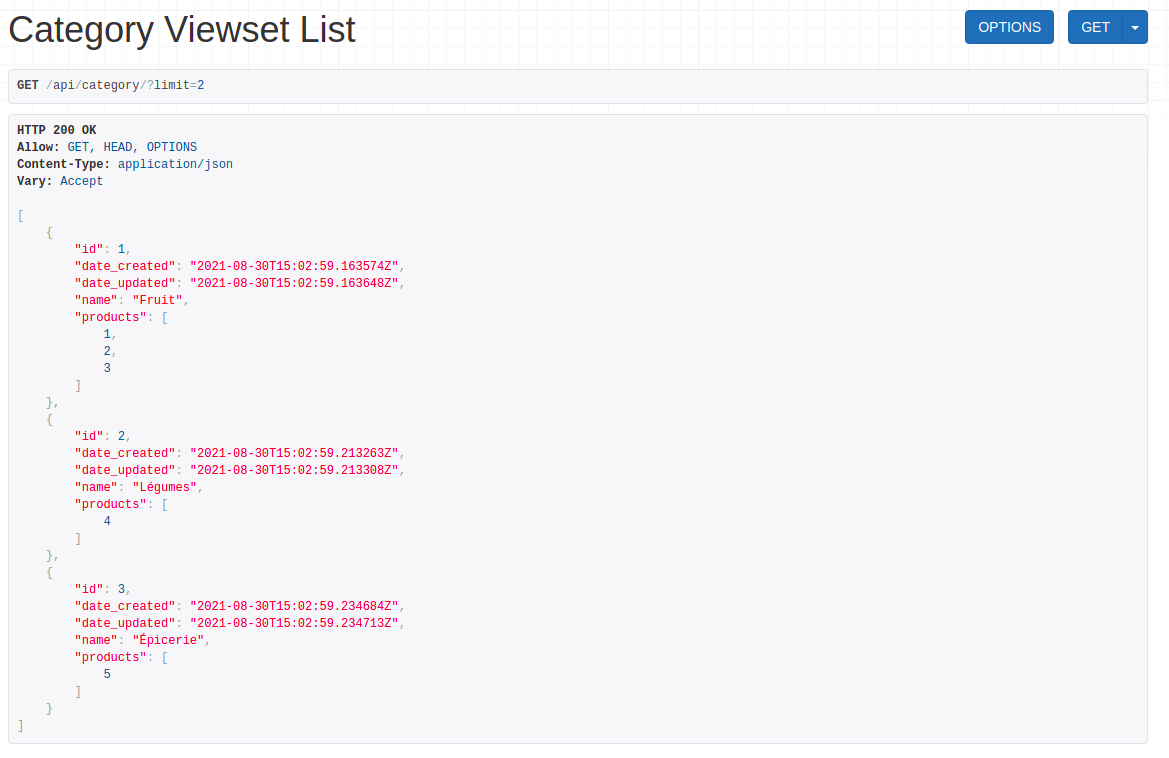
\includegraphics[width=12cm]{images/image12.png}
\end{center}

Cependant, un problème persiste, DRF affiche tous les produits de chaque catégorie, alors que nous voudrions n'afficher que ceux qui sont {\em actifs}. Pour cela, nous pouvons redéfinir notre attribut de classe {\tt products}  avec un {\tt SerializerMethodField}  qui nous donne alors la possibilité de {\em filtrer les produits à retourner}.
\begin{minted}[
mathescape,
framesep=2mm,
baselinestretch=1.2,
fontsize=\footnotesize,
bgcolor=LightGray,
%linenos
]{python}
class CategorySerializer(serializers.ModelSerializer):

    # En utilisant un `SerializerMethodField', il est nécessaire d'écrire une méthode
    # nommée 'get_XXX' où XXX est le nom de l'attribut, ici 'products'
    products = serializers.SerializerMethodField()

    class Meta:
        model = Category
        fields = ['id', 'date_created', 'date_updated', 'name', 'products']

    def get_products(self, instance):
        # Le paramètre 'instance' est l'instance de la catégorie consultée.
        # Dans le cas d'une liste, cette méthode est appelée autant de fois qu'il y a
        # d'entités dans la liste

        # On applique le filtre sur notre queryset pour n'avoir que les produits actifs
        queryset = instance.products.filter(active=True)
        # Le serializer est créé avec le queryset défini et toujours défini en tant que many=True
        serializer = ProductSerializer(queryset, many=True)
        # la propriété '.data' est le rendu de notre serializer que nous retournons ici
        return serializer.data
\end{minted}

\begin{center}
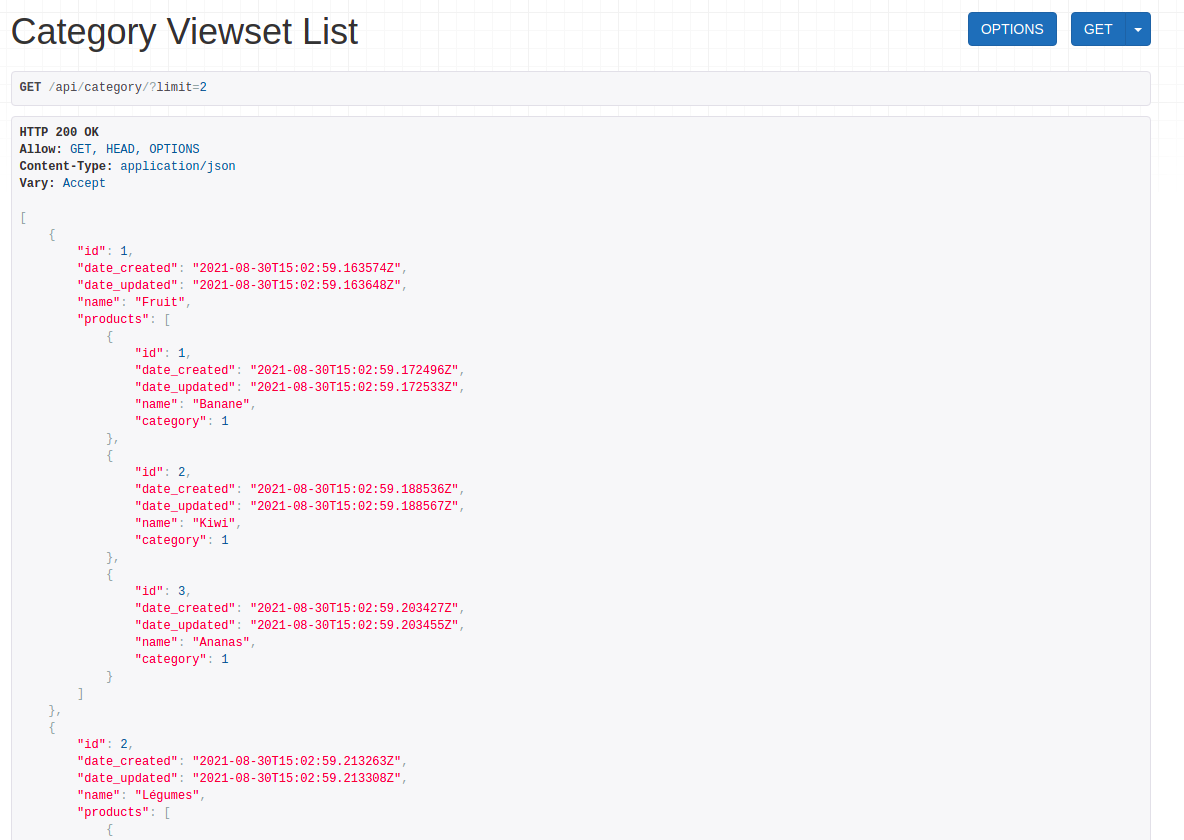
\includegraphics[width=12cm]{images/image13.png}
\end{center}
Nous pouvons constater qu'à présent les produits retournés sont bien seulement des produits actifs.

\subsubsection*{Et si on lançait nos tests après le développement de cette feature ?}
Oups, c’est cassé ! Et c’est tout à fait {\color{monOrange}normal}.

Une API se doit d’être minutieusement {\color{monOrange}testée}, car les retours de ces endpoints sont souvent garants du bon fonctionnement des applications clientes. L’ajout d’un attribut dans un endpoint ne pose en général aucun problème, mais le {\color{monOrange}retrait} d’un attribut peut avoir des conséquences plus importantes.

Imaginons que l’application mobile de notre site utilise l’attribut price  de nos articles, et que nous décidions de le {\color{monOrange}retirer} pour le déplacer ailleurs. Les applications mobiles ne pourraient pas alors afficher de prix tant qu’ils ne déploient pas eux-mêmes une nouvelle version de leur application qui utilise le {\color{monOrange}nouvel attribut}.

\subsubsection*{Mais ça fait beaucoup de données tout ça pour un seul endpoint, non ?}
Pour limiter les données retournées, il est possible de mettre en place une {\color{monOrange}pagination}. Faisons-le ensemble !
\subsection{Ajoutez de la pagination}
Mettre en place une pagination dès la création d’une API est une bonne pratique, car en limitant le nombre d’entités retournées, cela permet :
\begin{itemize}
\item De réduire le temps de réponse, surtout si le calcul de certains attributs est coûteux ;
\item Aux applications clientes de ne pas récupérer toutes les informations si elles ne se servent que d’une seule partie ;
\item D’éviter la modification des applications clientes par la suite, car la pagination impose certains attributs.
\end{itemize}
\begin{center}
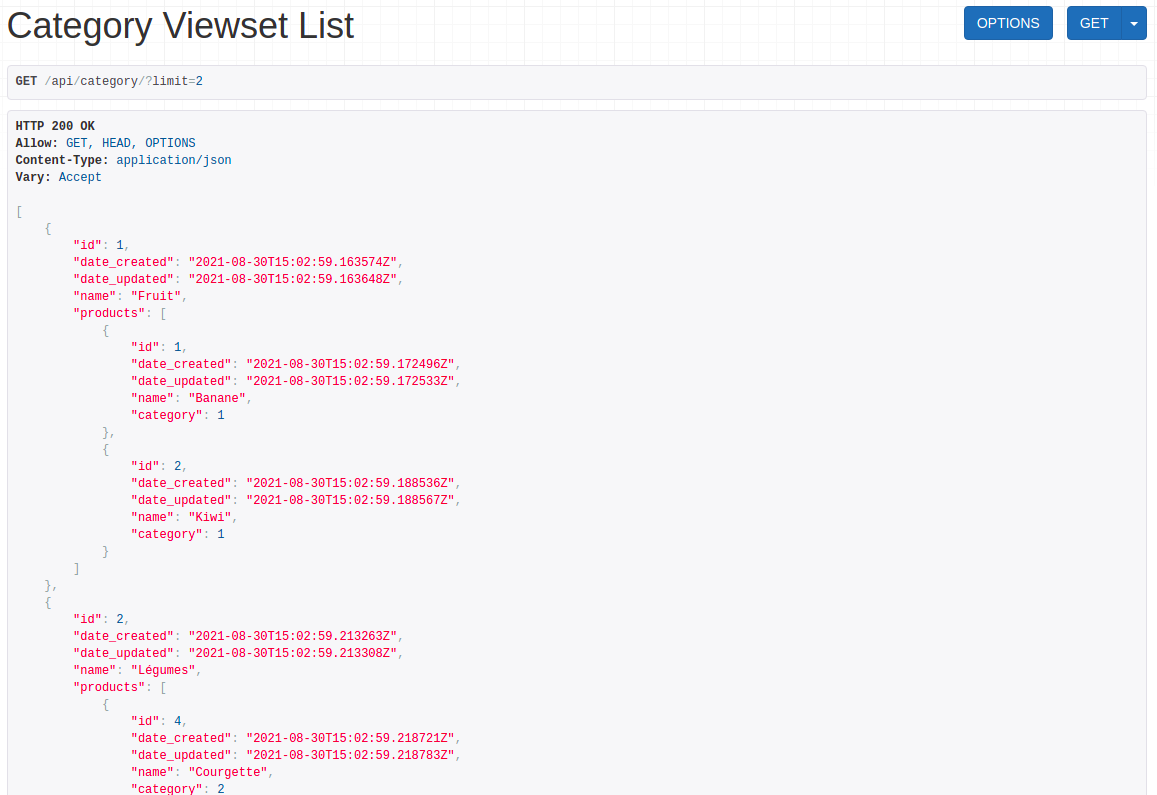
\includegraphics[width=12cm]{images/image14.png}
\end{center}
La pagination indique les informations suivantes :
\begin{itemize}
\item {\tt count  :} le nombre total d’éléments ;
\item {\tt next  :} l’URL de l’endpoint pour obtenir la page suivante ;
\item {\tt previous  :} l’URL de l’endpoint pour obtenir la page précédente ;
\item {\tt results  :} les données réelles utilisables.
\end{itemize}
\begin{theorem}
Lorsque les applications clientes sont réalisées en interne, il est important de bien communiquer avec ses équipes afin de savoir quelles sont les données qui leurs sont importantes, et dans quelles conditions. Le résultat de ces échanges vous donnera les meilleures pistes pour savoir quelles données retourner, et sous quel format.
\end{theorem}
Je vous propose de mettre en place le même mécanisme d’imbrication sur le serializer de produits, pour que les applications clientes puissent récupérer d’un coup les produits et leurs articles actifs.

Pour réaliser cela, vous pouvez partir de la branche \href{https://github.com/OpenClassrooms-Student-Center/7192416\_APIs\_DRF/tree/P2C1\_exercice}{P2C1\_exercice}. Elle contient déjà ce que nous venons de faire ensemble. Une solution est proposée sur la branche \href{https://github.com/OpenClassrooms-Student-Center/7192416\_APIs\_DRF/tree/P2C1\_solution}{P2C1\_solution}.
\begin{minted}[
mathescape,
framesep=2mm,
baselinestretch=1.2,
fontsize=\footnotesize,
bgcolor=LightGray,
%linenos
]{python}
from rest_framework import serializers
from shop.models import Category,Product,Article
 
class ArticleSerializer(serializers.ModelSerializer):
    class Meta:
        model = Article 
        fields = ['id', 'date_created', 'date_updated','name','description','active','price']

class ProductSerializer(serializers.ModelSerializer):
    articles=serializers.SerializerMethodField()
    class Meta:
        model = Product
        fields = ['id', 'date_created', 'date_updated','name','category','articles']  
          
    def get_articles(self,instance):
        queryset = instance.articles.filter(active=True)  
        serializer = ArticleSerializer(queryset,many=True) 
        return serializer.data 
         
class CategorySerializer(serializers.ModelSerializer):
    products=serializers.SerializerMethodField()
    class Meta:
        model = Category
        fields = ['id', 'date_created', 'date_updated' ,'name','products']  
    def get_products(self,instance):
        queryset = instance.products.filter(active=True)  
        serializer = ProductSerializer(queryset,many=True) 
        return serializer.data        
\end{minted}
\begin{center}
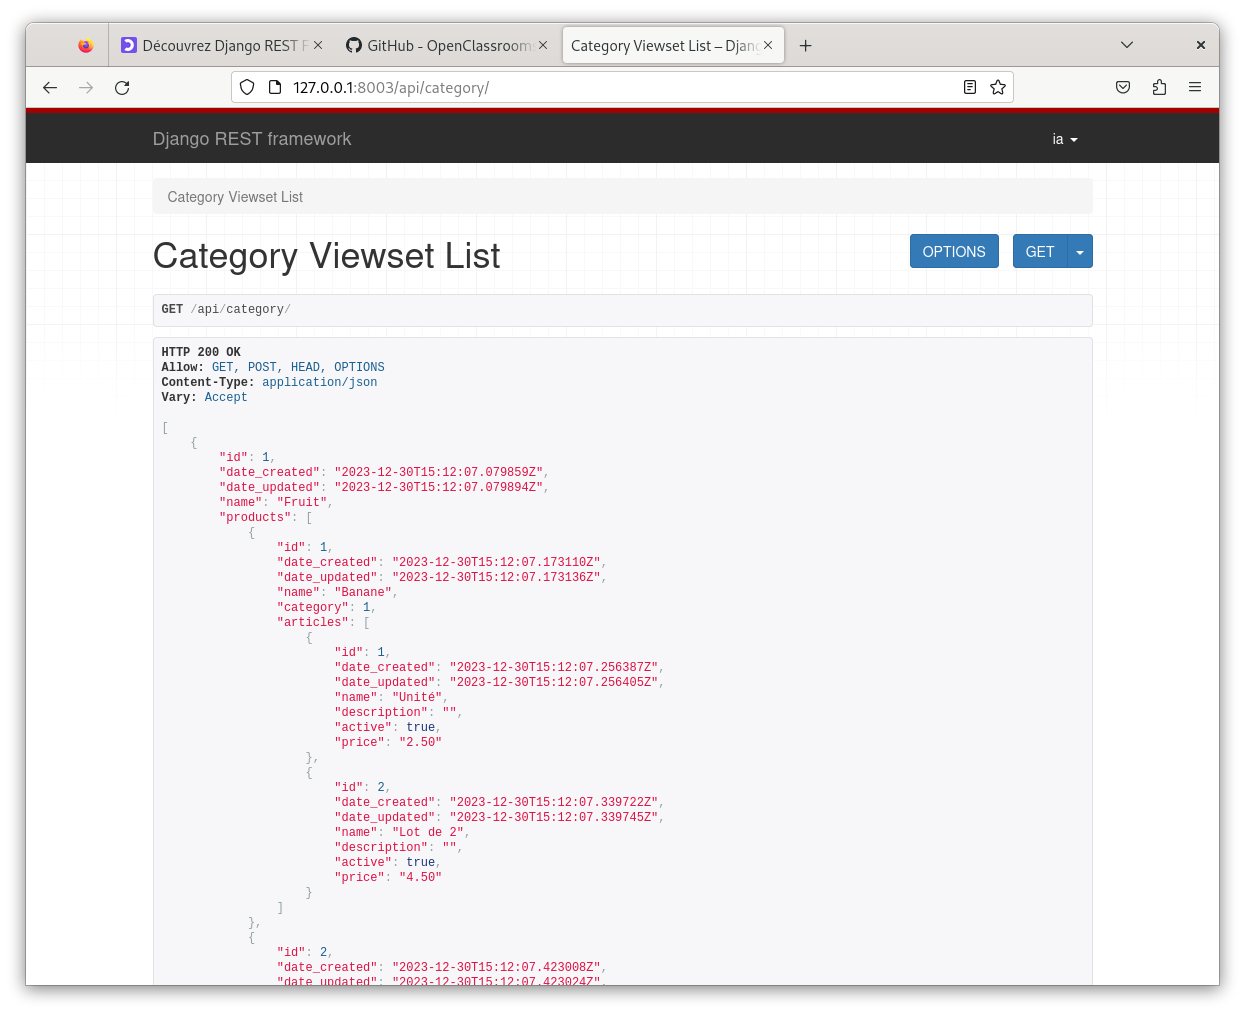
\includegraphics[width=12cm]{images/image16.png}
\end{center}
\subsubsection*{En résumé}
\begin{enumerate}
\item Imbriquer des serializers permet d’obtenir plus d’informations en un seul appel.
\item Il est possible d’appliquer des filtres sur un attribut du serializer en utilisant un {\tt SerializerMethodField}.
\item Toute modification d’un endpoint entraîne l’adaptation d’un test.
\item Il est bien de rapidement mettre en place une pagination sur une API.
\end{enumerate}

{\em Maintenant que nous avons optimisé le nombre d’appels de notre API, voyons comment différencier les informations retournées en liste ou en détail – vous me suivez au prochain chapitre ? C’est parti !}
\section{Différenciez les informations de liste et de détail}
\subsection{Retournez plus d’informations dans le détail}
Très souvent, les données en retour sont différentes selon qu’on consulte un endpoint de liste ou un endpoint de détail. En règle générale, les listes sont appelées pour être affichées. Lorsque l’utilisateur sélectionne un des éléments qui la composent, alors un autre appel est réalisé par l’application cliente afin d’obtenir plus d’informations. Cela permet de {\em réduire les temps de réponse} en ne retournant que les informations utiles.

Dans notre cas, la liste des catégories est bien trop complète pour l’usage qui doit en être fait, et nous allons donc réduire les informations de liste, en conservant toutes nos données actuelles dans l'endpoint de détail d’une catégorie.
\subsection{Améliorez le rendu du détail d’un endpoint}
Améliorons notre endpoint de catégories en ne retournant que les informations {\em minimales}, dans le cas d’une liste, et {\em détaillées}, lorsque nous consultons une catégorie spécifique.

DRF nous permet au travers de ses viewsets de redéfinir la méthode {\tt get\_serializer\_class}  qui, elle, détermine le serializer à utiliser. Par défaut, le serializer retourné est celui défini sur l’attribut de classe {\tt serializer\_class}  du viewset.

Lorsqu’une requête entre dans notre API, les viewsets définissent un attribut action  qui correspond à l’{\em action} que l’{\em application client} est en train de réaliser. Elle peut être :
\begin{itemize}
\item {\tt list :} appel en GET  sur l’URL de liste ;
\item {\tt retrieve :} appel en GET  sur l’URL de détail (qui comporte alors un identifiant) ;
\item {\tt create :} appel en POST  sur l’URL de liste ;
\item {\tt update :} appel en PUT  sur l’URL de détail ;
\item {\tt partial\_update :} appel en PATCH  sur l’URL de détail ;
\item {\tt destroy :} appel en DELETE  sur l’URL de détail.
\end{itemize}
\begin{minted}[
mathescape,
framesep=2mm,
baselinestretch=1.2,
fontsize=\footnotesize,
bgcolor=LightGray,
%linenos
]{python}
class CategoryViewset(ReadOnlyModelViewSet):
 
    serializer_class = CategoryListSerializer
    # Ajoutons un attribut de classe qui nous permet de définir notre serializer de détail
    detail_serializer_class = CategoryDetailSerializer
 
    def get_queryset(self):
        return Category.objects.filter(active=True)
 
    def get_serializer_class(self):
    # Si l'action demandée est retrieve nous retournons le serializer de détail
        if self.action == 'retrieve':
            return self.detail_serializer_class
        return super().get_serializer_class()
\end{minted}
\begin{center}
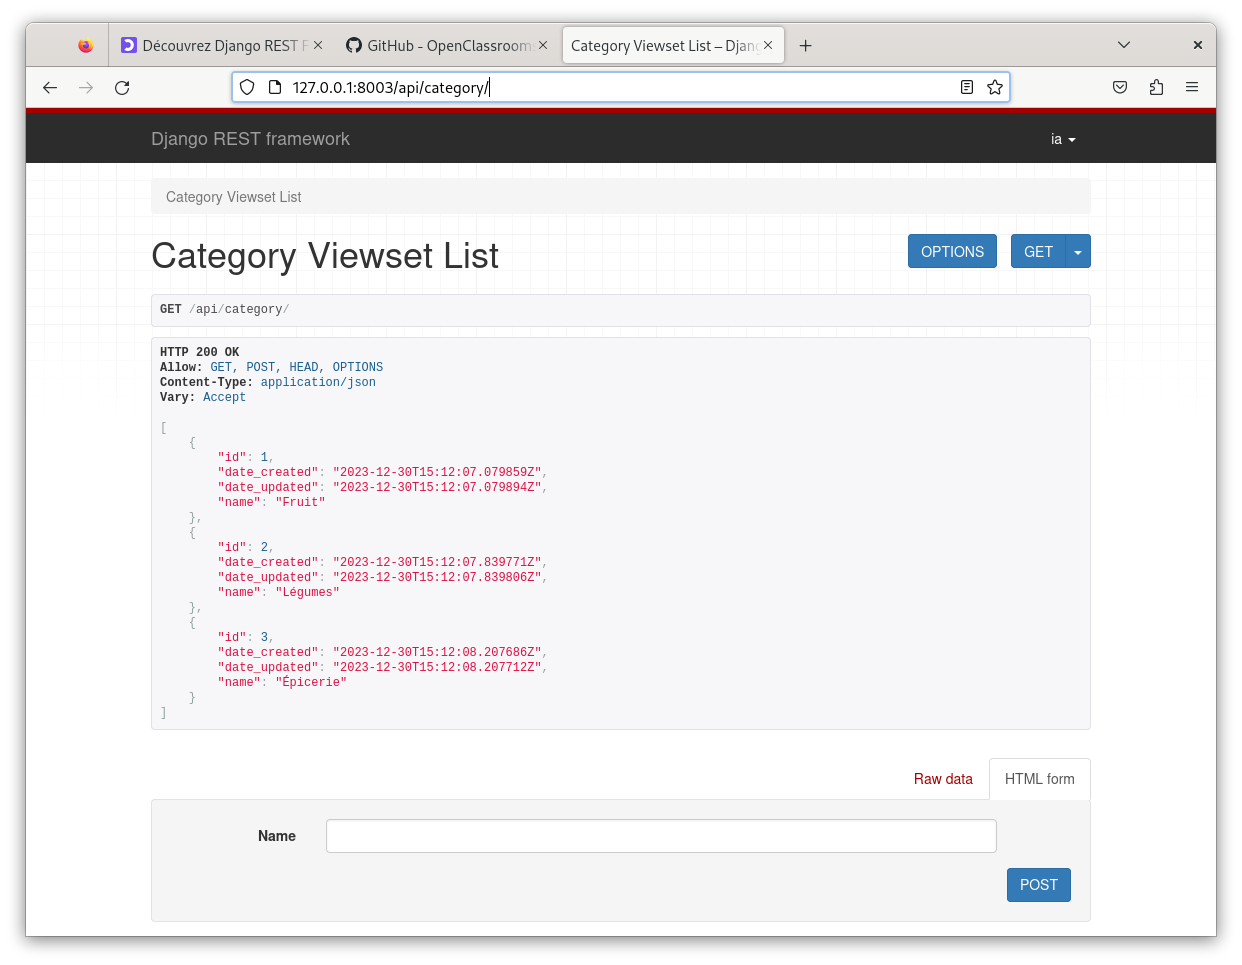
\includegraphics[width=12cm]{images/image17.png}
\end{center}
\begin{center}
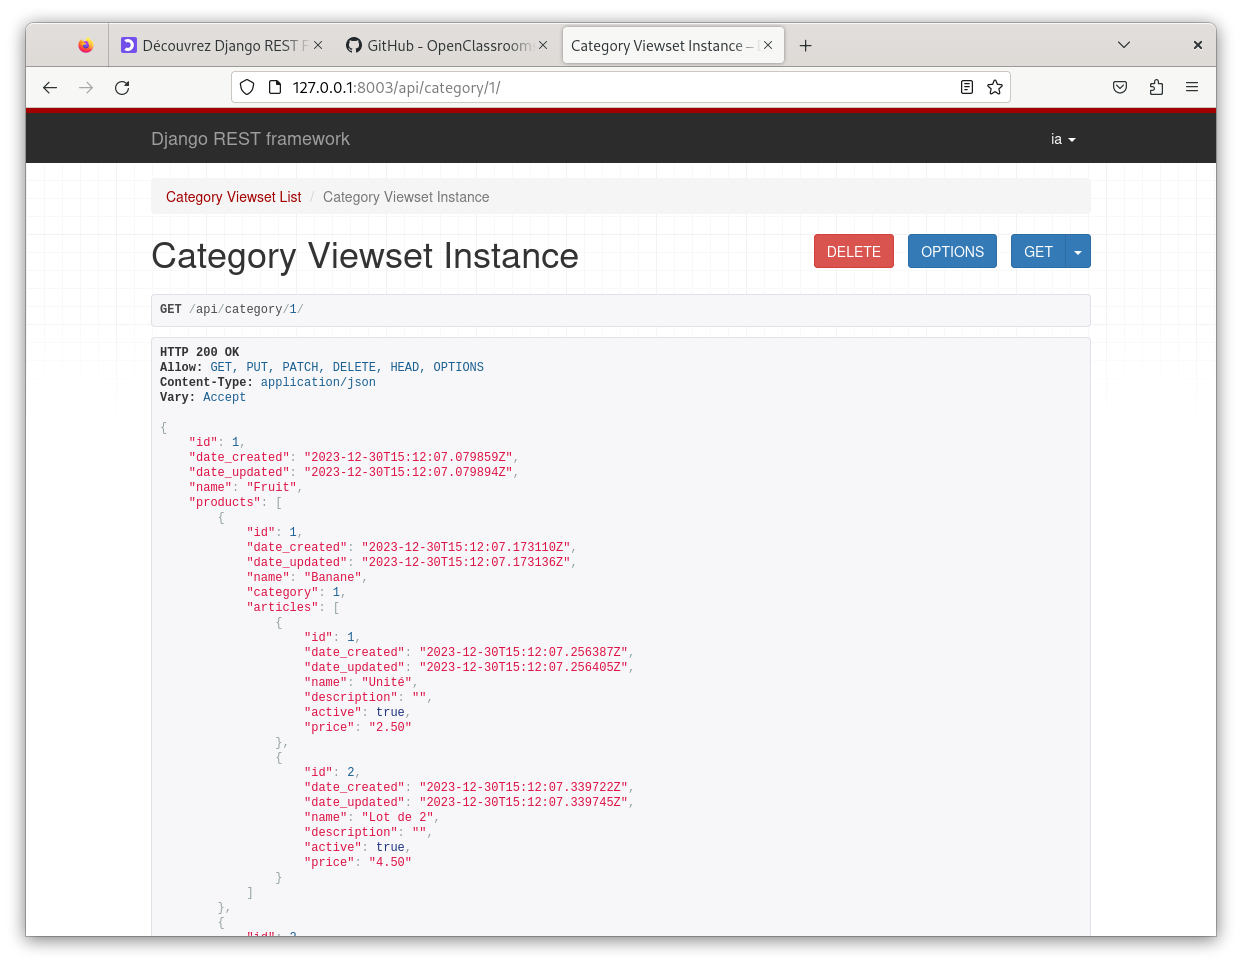
\includegraphics[width=12cm]{images/image18.png}
\end{center}

\subsubsection*{Exemple}
À vous à présent, faites de même et améliorez l'endpoint de produits pour que la liste reste succincte, et que le détail retourne plus d’informations. Pour réaliser cela, vous pouvez partir de la branche \href{https://github.com/OpenClassrooms-Student-Center/7192416\_APIs\_DRF/tree/P2C2\_exercice}{P2C2\_exercice}. Elle contient déjà ce que nous venons de faire ensemble. Une solution est proposée sur la branche \href{https://github.com/OpenClassrooms-Student-Center/7192416\_APIs\_DRF/tree/P2C1\_solution}{P2C2\_solution}.

\subsubsection*{En résumé}
\begin{enumerate}
\item L’action réalisée est définie dans l’attribut {\tt action}  des viewsets, et permet de savoir précisément l’action en cours.
\item Il est possible de définir un serializer différent pour chaque action.
\item Les mixins sont une bonne façon de gérer les différents serializers à utiliser, car cette opération est très courante.
\item Utiliser différents serializers contribue à améliorer les performances de l’API.
\end{enumerate}
{\em Dissocier les serializers de liste et de détail nous permettrait par exemple d’inclure les produits et articles dans le détail d’une catégorie. N’hésitez pas à expérimenter. }

\section{Ajoutez de l’interaction avec les actions}
\subsection{Ne soyez pas trop actif !}
\subsubsection*{Une action, on a déjà parlé de ça, non ?}
Nous avons parlé du paramètre action  des Viewsets, mais dans ce chapitre nous allons voir le {\color{monOrange}décorateur} {\tt action},  fourni par DRF, qui permet de réaliser d’autres types d’actions que les classiques du CRUD, comme {\em Demander en ami}, {\em S’abonner à un fil d’actualité} ou {\em Publier un article}.

Vous devez penser  {\color{monOrange}Action} chaque fois qu’un besoin fait référence à une entité, mais que le verbe ne correspond pas à un élément du CRUD. Par exemple, dans {\em Nous souhaitons que nos visiteurs puissent liker des publications}, l’ {\color{monOrange}entité est la publication} et l’ {\color{monOrange}action est liker}.

Une action se crée dans DRF en mettant en place le décorateur {\tt action}  sur une méthode d’un Viewset. Les paramètres suivants sont disponibles :
\begin{itemize}
\item {\tt methods}  est la liste des méthodes HTTP qui appellent cette action, parmi GET, POST, PATCH, PUT, DELETE.
\item {\tt detail}  est un booléen qui précise si l’action est disponible sur l’URL de liste ou de détail.
\item {\tt url\_path}  permet de déterminer l’URL qui sera ajoutée à la fin de l'endpoint de liste ou de détail. S'il n’est pas précisé, alors le nom de la méthode est utilisé.
\end{itemize}
Pour notre boutique en ligne, on pourrait imaginer une action qui permette d’{\color{monOrange}activer} ou de désactiver une catégorie.

\subsubsection*{Mais on ne pourrait pas juste faire un PATCH sur la catégorie pour mettre active  à False  ?}
On pourrait effectivement, mais nous aimerions également désactiver tous les produits qui composent cette catégorie. Plutôt que de laisser les applications clientes faire tous ces appels, mettons-leur à disposition {\color{monOrange}un seul endpoint} qui réalise cela. D’ailleurs, vous savez quoi ? On va le faire tout de suite… ;)
\subsection{Soyez actif quand même !}
Les actions se mettent en place sur les Viewsets, alors allons modifier notre {\tt CategoryViewset}  pour lui ajouter une action {\tt disable}  que nous souhaitons accessible en POST.
\begin{minted}[
mathescape,
framesep=2mm,
baselinestretch=1.2,
fontsize=\footnotesize,
bgcolor=LightGray,
%linenos
]{python}
 @transaction.atomic
    @action(detail=True, methods=['post'])
    def disable(self, request, pk):
        # Nous avons défini notre action accessible sur la méthode POST seulement
        # elle concerne le détail car permet de désactiver une catégorie

        # Nous avons également mis en place une transaction atomique car plusieurs requêtes vont être exécutées
        # en cas d'erreur, nous retrouverions alors l'état précédent

        # Désactivons la catégorie
        category = self.get_object()
        category.active = False
        category.save()

        # Puis désactivons les produits de cette catégorie
        category.products.update(active=False)

        # Retournons enfin une réponse (status_code=200 par défaut) pour indiquer le succès de l'action
        return Response()
\end{minted}
Ainsi, la réalisation d’un POST sur l'endpoint \href{http://127.0.0.1:8000/api/category/2/disable/}  aura pour effet de :
\begin{enumerate}
\item Désactiver la {\color{monOrange}catégorie}, ce qui ne rendra plus visible la catégorie sur l'endpointhttp://127.0.0.1:8000/api/category/.
\item Désactiver {\color{monOrange}les produits de cette catégorie}, ce qui ne rendra plus visible ces produits sur l'endpoint http://127.0.0.1:8000/api/product/.
\end{enumerate}
\begin{theorem}
Il est toujours préférable de rapprocher le code métier du model afin de pouvoir l’exécuter plus facilement. Faisons cela, et notre action en sera alors simplifiée.
\end{theorem}
Ajoutons une méthode {\tt disable}  à notre model {\tt Category}  :
\begin{minted}[
mathescape,
framesep=2mm,
baselinestretch=1.2,
fontsize=\footnotesize,
bgcolor=LightGray,
%linenos
]{python}
class Category(models.Model):
 
    date_created = models.DateTimeField(auto_now_add=True)
    date_updated = models.DateTimeField(auto_now=True)
 
    name = models.CharField(max_length=255)
    active = models.BooleanField(default=False)
 
    @transaction.atomic
    def disable(self):
        if self.active is False:
        # Ne faisons rien si la catégorie est déjà désactivée
            return
        self.active = False
        self.save()
        self.products.update(active=False)
\end{minted}
\begin{theorem}
Vous remarquerez que nous avons déplacé la transaction atomique sur la méthode du model, elle n’est donc plus nécessaire sur l’action du Viewset.
\end{theorem}
\begin{minted}[
mathescape,
framesep=2mm,
baselinestretch=1.2,
fontsize=\footnotesize,
bgcolor=LightGray,
%linenos
]{python}
class MultipleSerializerMixin:
    # Un mixin est une classe qui ne fonctionne pas de façon autonome
    # Elle permet d'ajouter des fonctionnalités aux classes qui les étendent

    detail_serializer_class = None

    def get_serializer_class(self):
        # Notre mixin détermine quel serializer à utiliser
        # même si elle ne sait pas ce que c'est ni comment l'utiliser
        if self.action == 'retrieve' and self.detail_serializer_class is not None:
            # Si l'action demandée est le détail alors nous retournons le serializer de détail
            return self.detail_serializer_class
        return super().get_serializer_class()

class CategoryViewset(MultipleSerializerMixin, ReadOnlyModelViewSet):
 
    serializer_class = CategoryListSerializer
    detail_serializer_class = CategoryDetailSerializer
 
    @action(detail=True, methods=['post'])
    def disable(self, request, pk):
        # Nous pouvons maintenant simplement appeler la méthode disable
        self.get_object().disable()
        return Response()
\end{minted}
\begin{center}
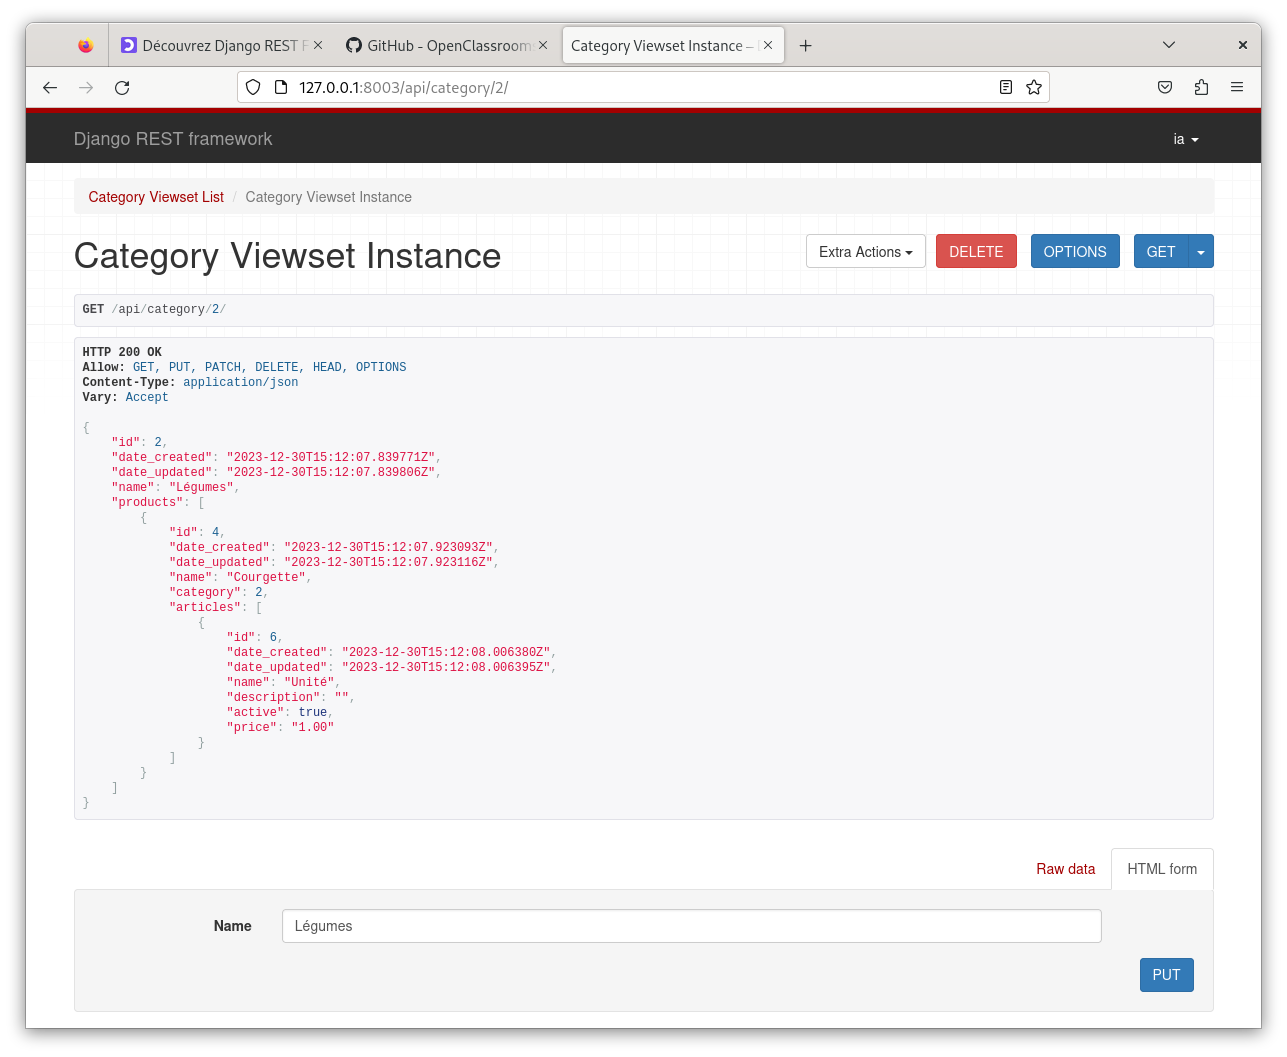
\includegraphics[width=12cm]{images/image19.png}
\end{center}
\begin{center}
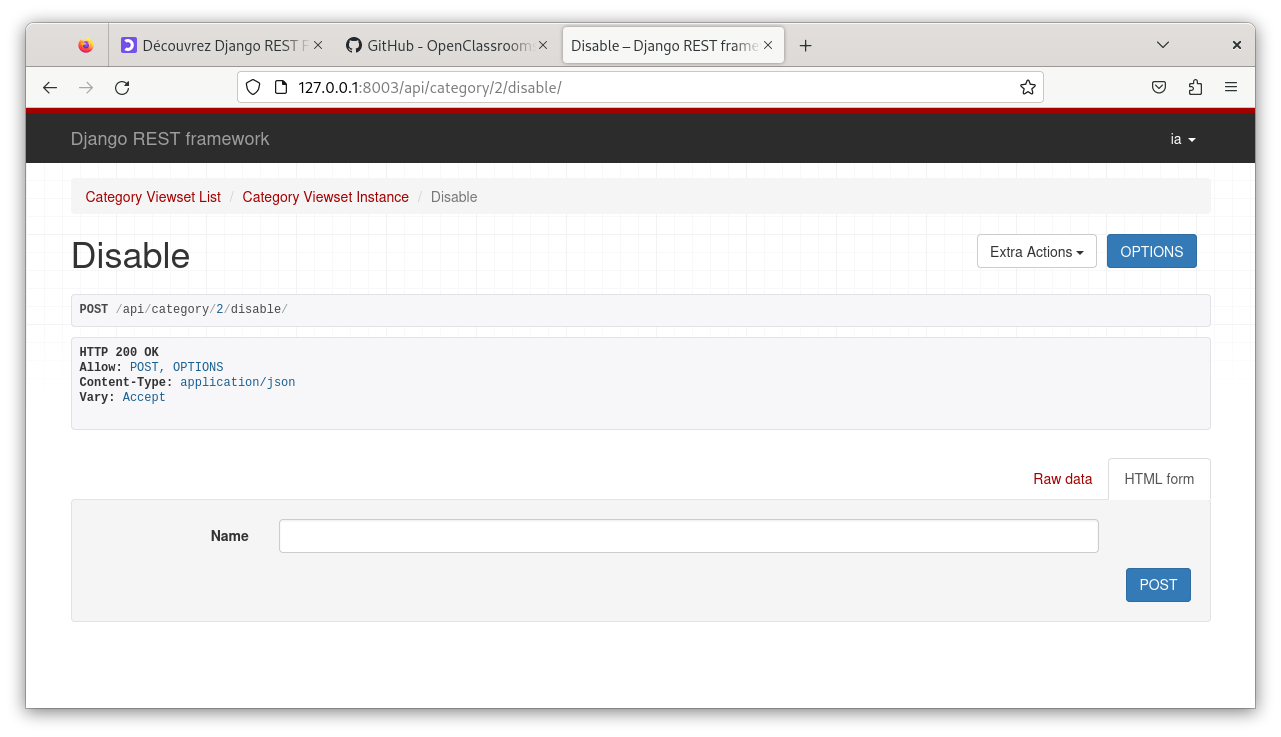
\includegraphics[width=12cm]{images/image20.png}
\end{center}


\begin{theorem}
Cette modification ne change en rien le fonctionnement de notre API, mais permet une {\color{monOrange}lecture} plus claire du code. L’action ne fait qu'appeler une méthode de notre model {\tt Category}.
\end{theorem}

\subsubsection*{Exercice}
Mettons en place le même système pour {\color{monOrange}désactiver un produit} qui {\color{monOrange}désactive également les articles associés}. Nous pourrions également améliorer la désactivation d’une catégorie en désactivant les articles de chaque produit.

Pour réaliser cela, vous pouvez partir de la branche \href{https://github.com/OpenClassrooms-Student-Center/7192416\_APIs\_DRF/tree/P2C3\_exercice}{P2C3\_exercice}. Elle contient déjà ce que nous venons de faire ensemble. Une solution est proposée sur la branche \href{https://github.com/OpenClassrooms-Student-Center/7192416\_APIs\_DRF/tree/P2C3\_solution}{P2C3\_solution}.
\subsubsection*{En résumé}
\begin{enumerate}
\item Il est possible de créer d’autres actions en dehors de celles du CRUD.
\item DRF met à disposition un décorateur {\tt action}  qui permet de créer de nouvelles actions.
\item Les actions peuvent être mises en place sur les URL de liste et de détail d’un endpoint.
\item Les actions peuvent utiliser n’importe quelle méthode HTTP (GET, POST, PATCH, DELETE…).
\end{enumerate}
{\em Les actions servent à gérer des morceaux de logique métier, et ainsi à éviter aux applications clientes de les gérer, car elles pourraient les gérer différemment. Le fait d’ajouter un article au panier d’un utilisateur est un bon exemple d’action qui ne peut être réalisé que d’une seule façon, son traitement doit donc être réalisé par le serveur et non les applications clientes. Dans le chapitre suivant, vous découvrirez comment valider les données transmises par ces actions !}

%%%%%%%%%%%%%%%%%%%%%%%%%%%%%%%%%%%%%%%%%%%%%%%
\section{Validez les données}
\subsection{Ne permettez pas la création de tout et n’importe quoi}
Attaquons-nous à présent à un autre sujet : {\color{monOrange}la création d’entités} et plus précisément de catégories, dans notre cas.

Notre endpoint actuel permet la lecture seulement, car il est destiné aux visiteurs de notre boutique. Nous allons très vite en mettre un second en place, qui sera dédié aux {\color{monOrange}administrateurs} qui, eux, auront la possibilité de {\color{monOrange}créer, modifier et supprimer} des données. La création d’entité impose d’effectuer certains contrôles qui sont généralement de deux types :
\begin{enumerate}
\item Les contrôles {\color{monOrange}sur un champ}, comme par exemple vérifier que le nom d’une catégorie n'existe pas déjà, et ainsi éviter les doublons.
\item Les contrôles {\color{monOrange}multichamps}, comme la vérification que les deux mots de passe saisis à l’inscription sont les mêmes.
\end{enumerate}
DRF nous permet de réaliser ces deux types de contrôles au travers de la réécriture de méthodes sur le serializer :
\begin{itemize}
\item {\tt validate\_XXX}  où XXX est le nom du champ à valider ;
\item {\tt validate}  qui permet un contrôle global sur tous les champs du serializer.
\end{itemize}
N’attendons pas plus longtemps pour mettre en place l'endpoint et les contrôles qui l’accompagnent. ;)

\subsection{Validez les données d’un champ}
Commençons tout de suite par la mise en place du nouvel endpoint sur l’URL \href{http://127.0.0.1:8000/api/admin/category/}  qui, comme son nom l’indique, servira à administrer les catégories.
\subsubsection*{Pourquoi ne pas utiliser l’endpoint déjà existant ?}
 Dans les endpoints d’administration :
\begin{itemize}
\item Des serializers différents sont utilisés et les données retournées diffèrent ;
\item Certains accès peuvent également être limités à certaines personnes authentifiées.
\end{itemize}
 
Dans le cadre de notre boutique, nous avons décidé de {\color{monOrange}définir nos endpoints} en fonction des {\color{monOrange}acteurs} qui les utilisent. Créons {\color{monOrange}notre nouvel endpoint d’administration} qui cette fois-ci étend {\tt ModelViewset}  et non plus {\tt ReadOnlyViewset}. Celui-ci ne doit pas avoir de limitation sur les catégories actives, car il s’agit d’un endpoint d’administration.
\begin{minted}[
mathescape,
framesep=2mm,
baselinestretch=1.2,
fontsize=\footnotesize,
bgcolor=LightGray,
%linenos
]{python}
class AdminCategoryViewset(MultipleSerializerMixin, ModelViewSet):
 
    serializer_class = CategoryListSerializer
    detail_serializer_class = CategoryDetailSerializer
 
    def get_queryset(self):
        return Category.objects.all()
\end{minted}
Puis définissons notre nouvel endpoint en le {\color{monOrange}déclarant auprès de notre routeur}.

\begin{minted}[
mathescape,
framesep=2mm,
baselinestretch=1.2,
fontsize=\footnotesize,
bgcolor=LightGray,
%linenos
]{python}
router.register('admin/category', AdminCategoryViewset, basename='admin-category')
\end{minted}
Vérifions que notre endpoint est bien fonctionnel sur l’URL  
\begin{center}
\url{http://127.0.0.1/api/admin/category}
\end{center}
Maintenant que nous utilisons un {\tt Viewset}, {\color{monOrange}la création de catégorie est possible}. C’est à la création que sert ce formulaire en nous permettant d'effectuer des actions POST. Les actions de mise à jour et de suppression sont disponibles sur les URL de détail des catégories.

Validons à présent nos données, sans oublier que la création d’un doublon de catégorie ne doit pas être permis. Il nous faut pour cela modifier notre serializer de liste, car c’est lui qui est utilisé pour l’action create  .

La {\color{monOrange}validation d’un champ} unique se fait en écrivant la méthode {\tt validate\_XXX}  où XXX  est le nom du champ. Dans notre cas, {\color{monOrange}validate\_name}  :
\begin{minted}[
mathescape,
framesep=2mm,
baselinestretch=1.2,
fontsize=\footnotesize,
bgcolor=LightGray,
%linenos
]{python}
class CategoryListSerializer(serializers.ModelSerializer):
 
    class Meta:
        model = Category
        fields = ['id', 'date_created', 'date_updated', 'name']
 
    def validate_name(self, value):
        # Nous vérifions que la catégorie existe
        if Category.objects.filter(name=value).exists():
        # En cas d'erreur, DRF nous met à disposition l'exception ValidationError
            raise serializers.ValidationError('Category already exists')
        return value
\end{minted}
Si nous tentons à présent de créer une catégorie qui existe déjà, une réponse en 400 avec des données contenant la nature de l’erreur sont renvoyées.
\begin{center}
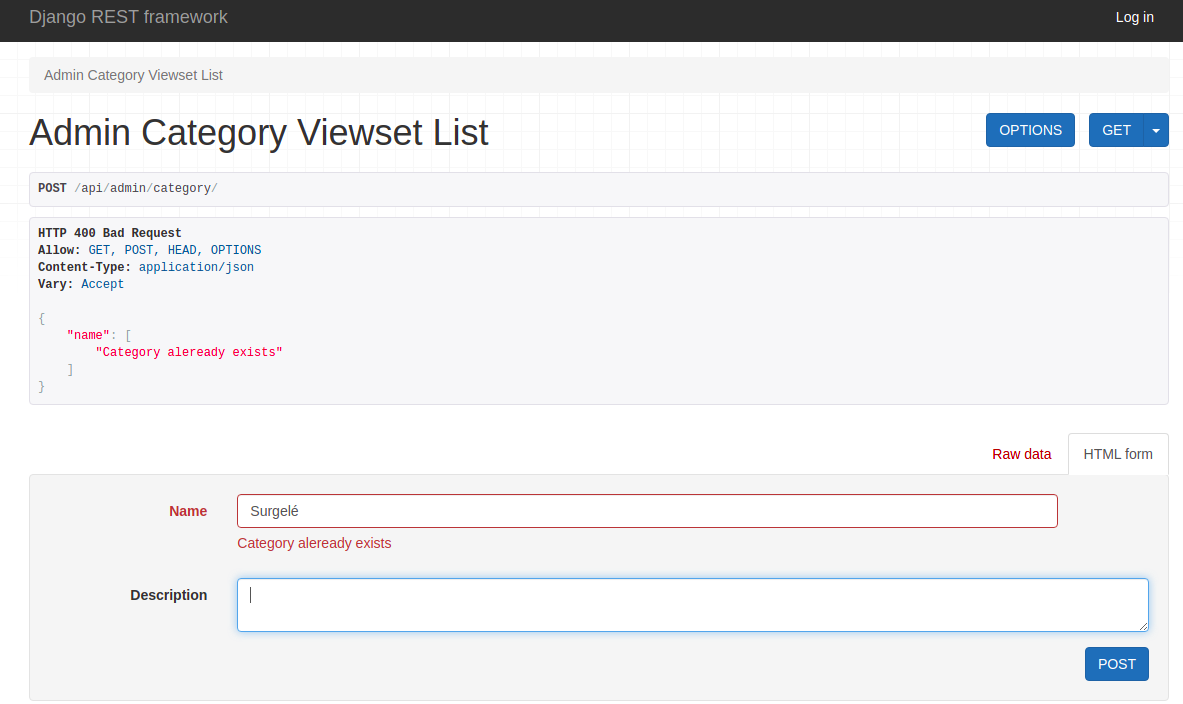
\includegraphics[width=12cm]{images/image21.png}
\end{center}
La validation de champ unique permet d’effectuer plein de {\color{monOrange}contrôles}, tant qu’ils sont effectués sur ce champ précis. On pourrait imaginer un système de filtre de mots pour un forum, par exemple.

\subsection{Mettez en place une validation multiple}
Pour notre boutique, nous souhaitons optimiser le référencement et avoir un rappel du nom de la catégorie également présent dans la description. Nous pouvons effectuer automatiquement ce contrôle au travers d’une validation multiple.

La validation entre champs se fait au travers de la méthode {\tt validate}. Vérifions que le nom est bien présent dans la description :


\begin{minted}[
mathescape,
framesep=2mm,
baselinestretch=1.2,
fontsize=\footnotesize,
bgcolor=LightGray,
%linenos
]{python}
class CategoryListSerializer(serializers.ModelSerializer):
 
    class Meta:
        model = Category
        # Pensons à ajouter « description » à notre liste de champs
        fields = ['id', 'date_created', 'date_updated', 'name', 'description']
 
    def validate_name(self, value):
        if Category.objects.filter(name=value).exists():
            raise serializers.ValidationError('Category already exists')
        return value
 
    def validate(self, data):
        # Effectuons le contrôle sur la présence du nom dans la description
        if data['name'] not in data['description']:
        # Levons une ValidationError si ça n'est pas le cas
            raise serializers.ValidationError('Name must be in description')
        return data
\end{minted}
Nous pouvons alors constater que notre validation fonctionne si le nom de la catégorie n’est pas présent dans sa description.
\begin{center}
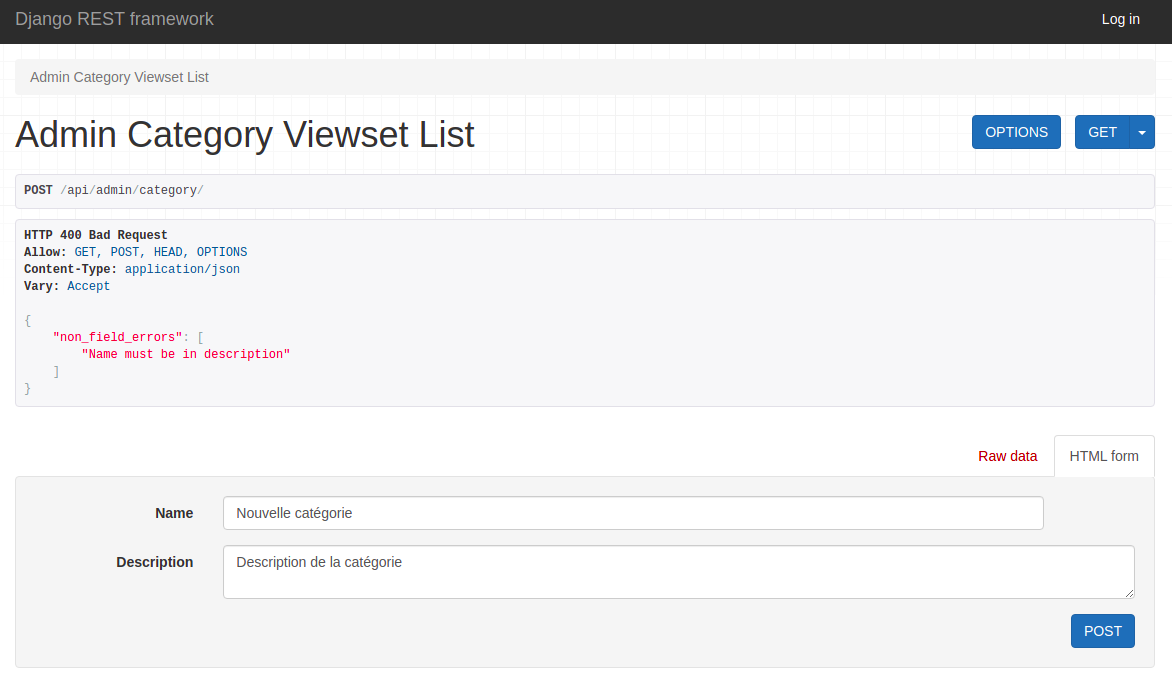
\includegraphics[width=12cm]{images/image22.png}
\end{center}

\subsubsection*{Exercice}
Mettons en place un endpoint d’administration des articles pour les administrateurs de la boutique. Certains contrôles doivent être effectués :
\begin{itemize}
\item Le {\color{monOrange}prix} doit être supérieur à 1€.
\item Le produit associé doit être {\color{monOrange}actif}.
\end{itemize}
Pour réaliser cela, vous pouvez partir de la branche \href{https://github.com/OpenClassrooms-Student-Center/7192416\_APIs\_DRF/tree/P2C4\_exercice}{P2C4\_exercice}. Elle contient déjà ce que nous venons de faire ensemble. Une solution est proposée sur la branche \href{https://github.com/OpenClassrooms-Student-Center/7192416\_APIs\_DRF/tree/P2C4\_solution}{P2C4\_solution}.

\subsubsection*{En résumé}
\begin{enumerate}
\item Utiliser un ModelViewset permet l’utilisation de l’ensemble des actions du CRUD.
\item La validation d’un champ se fait au travers de la méthode {\tt validate\_XXX}  du serializer.
\item La validation multichamp se fait au travers de la méthode {\tt validate}  du serializer.
\end{enumerate}
{\em La validation des données lors de la création et/ou la modification est un facteur clé pour assurer la cohérence des données, n’hésitez pas à valider toutes les données importantes. Maintenant, voyons comment tester les API externes avec les mocks – suivez-moi au prochain chapitre !}
\end{document}











    \chapter{Sécurisez votre API avec l’authentification}
    \documentclass[a4paper]{article}
 
% - taille de la fonte    : 10pt, 11pt, 12pt
% - recto ou recto-verso    : oneside, twoside
 
% Chargement d'extensions
%\usepackage[latin1]{inputenc}    
\usepackage[francais]{babel}    
\AtBeginDocument{\def\labelitemi{$\bullet$}}

\usepackage{amsmath}
\makeatletter
%%%%%%%%%%%%%%%%%%% debut fichier boiboites.sty %%%%%%%%%%%%%%%%%%%%%%
\RequirePackage{xkeyval}
\RequirePackage{tikz}
\RequirePackage{amssymb}

\define@key{boxedtheorem}{titlecolor}{\def\titlecolor{#1}}
\define@key{boxedtheorem}{titlebackground}{\def\titlebackground{#1}}
\define@key{boxedtheorem}{background}{\def\background{#1}}
\define@key{boxedtheorem}{titleboxcolor}{\def\titleboxcolor{#1}}
\define@key{boxedtheorem}{boxcolor}{\def\boxcolor{#1}}
\define@key{boxedtheorem}{thcounter}{\def\thcounter{#1}}
\define@key{boxedtheorem}{size}{\def\size{#1}}
\presetkeys{boxedtheorem}{titlecolor = black, titlebackground = white, background = white,%
                         titleboxcolor = black, boxcolor = black, thcounter=, size = .9\textwidth}{}

\newcommand{\couleurs}[1][]{%
    \setkeys{boxedtheorem}{#1}
    \tikzstyle{fancytitle} =[draw=\titleboxcolor, rounded corners, fill=\titlebackground,
                            text= \titlecolor]
    \tikzstyle{mybox} = [draw=\boxcolor, fill=\background, very thick,
                        rectangle, rounded corners, inner sep=10pt, inner ysep=20pt]
}


%Commande generique pour faire un joli encadre
\newsavebox{\boiboite}
\newcommand{\titre}{Titre}
\newenvironment{boite}[2][]%
    {%
    \renewcommand{\titre}{#2}
    \couleurs[#1]
    \begin{lrbox}{\boiboite}%
     \begin{minipage}[!h]{\size}
    }%
    {%
     \end{minipage}
    \end{lrbox}
    \begin{center}
    \begin{tikzpicture}
    \node [mybox] (box){\usebox{\boiboite}};
    \node[fancytitle, right=10pt] at (box.north west) {\titre};
    \end{tikzpicture}
    \end{center}
    }

\newcommand{\newboxedtheorem}[4][]{%
    \couleurs[#1]
    \@ifnotempty{#4}{%
      \@ifundefined{the#4}{\@ifundefined{\thcounter}{\newcounter{#4}}{%
      \newcounter{#4}[\thcounter ] } } { }%
    }
    \newenvironment{#2}[1][]{%
    \@ifnotempty{#4}{\refstepcounter{#4}}
    \begin{boite}[#1]{\textbf{#3\@ifnotempty{#4}{ \csname the#4\endcsname}}\@ifnotempty{##1}{
    (##1)}}
    }%
    {%
    \end{boite}
    }
}
%%%%%%%%%%%%%%%%%%%% end fichier boiboites.sty %%%%%%%%%%%%%%%%%%%%%%
\makeatother
\newboxedtheorem{theorem}{}{theorem}
%%%%%%%%%% hypertext

\usepackage{hyperref}
\hypersetup{
    colorlinks=true,
    linkcolor=blue,
    filecolor=magenta,      
    urlcolor=cyan,
    pdftitle={Overleaf Example},
    pdfpagemode=FullScreen,
    }

\urlstyle{same}

%%%%%%%%%%%%%%%%%%%%%%%%%%%
\usepackage{amsthm}
%\usepackage{amsmath}
\usepackage{amssymb}
\usepackage{mathrsfs}
\usepackage{graphicx}
\usepackage{geometry}
\usepackage{stmaryrd}
\usepackage{tikz}
\usetikzlibrary{patterns}

\usepackage[cache=false]{minted}
\usepackage{xcolor}
%\setbeamercolor{background canvas}{bg=lightgray}
\definecolor{LightGray}{gray}{0.9}
\definecolor{monOrange}{rgb}{0.97,0.35,0.04}
 \setlength{\parindent}{0pt}
% Informations le titre, le(s) auteur(s), la date
\title{Sécurisez votre API avec l’authentification}
\author{Ibrahim ALAME}
\date{\today}

\begin{document}
 
\maketitle
 %Mettez en place une API simple avec Django REST Framework
\section{Ajoutez l’authentification des utilisateurs}
\subsection{Découvrez JSON Web Token}
L’authentification permet de rendre certains endpoints {\color{monOrange}privés} et accessibles seulement aux utilisateurs authentifiés. Ce qui est bien le cas pour notre boutique en ligne !

Nous souhaitons que les endpoints utiles aux visiteurs soient publics, cependant nous souhaitons disposer d'{\color{monOrange}endpoints d’administration} auxquels seuls les administrateurs de la plateforme pourront avoir accès. Nous ne souhaitons pas permettre aux visiteurs de modifier le prix d’un article avant de l’acheter, par exemple.

Nous allons donc mettre en place un système d’authentification basé sur JWT et la librairie \href{https://www.django-rest-framework.org/api-guide/authentication/\#json-web-token-authentication}{Simple JWT} qui est préconisée par DRF.
\begin{theorem}
Il existe divers modes d'authentification, ceux préconisés par DRF sont disponibles sur sa {\color{monOrange}documentation} (en anglais).
\end{theorem}
JWT est le sigle de {\em JSON Web Token}, qui est un {\color{monOrange}jeton d’identification} communiqué entre un serveur et un client. Il permet l’échange de données sécurisées entre ces derniers.

Dans le cadre de l’authentification, le JWT est utilisé pour s’assurer de l’identité de la personne réalisant la requête. Lorsque le serveur reçoit une requête, il vérifie alors la validité du token et détermine l’utilisateur à l’initiative de la requête. Le JWT permet d’identifier l’{\color{monOrange}utilisateur} à l’origine de la requête et permet ainsi de {\color{monOrange}vérifier ses droits}.

\subsubsection*{Ça ressemble à quoi, un JWT ?}
Un JWT est constitué de 3 parties séparées par un point. Par exemple ce JWT : 

\begin{verbatim}
eyJ0eXAiOiJKV1QiLCJhbGciOiJIUzI1NiJ9.eyJ0b2tlbl90eXBlIjoicmVmcmVzaCIsImV
4cCI6MTYyODk0ODE0NSwianRpIjoiODBmZTA4MDkxM2UxNDBjYmEwMDU4YWY4YmM5NjllZjY
iLCJ1c2VyX2lkIjoxfQ.l31cs5pTApiR9R9s8pZaeyHIJuTmjcs07fxSqSpj1fQ
\end{verbatim} 


Chaque partie est encodée en base64, il est possible d’utiliser \href{https://jwt.io}{jwt.io} pour les déchiffrer :
\begin{itemize}
\item Le {\color{monOrange}header}, qui est en général constitué de deux attributs, indique le type de token et l'algorithme de chiffrement utilisé.
Une fois décodé :
\begin{minted}[
mathescape,
framesep=2mm,
baselinestretch=1.2,
%fontsize=\footnotesize,
bgcolor=LightGray,
%linenos
]{python}
{
    "typ": "JWT",
    "alg": "HS256"
}
\end{minted}
\item Le {\color{monOrange}payload} contient les informations utiles que nous souhaitons faire transiter entre le serveur et le client.
Une fois décodé :
\begin{minted}[
mathescape,
framesep=2mm,
baselinestretch=1.2,
%fontsize=\footnotesize,
bgcolor=LightGray,
%linenos
]{python}
{
    "token_type": "refresh",
    "exp": 1628948145,
    "jti": "80fe080913e140cba0058af8bc969ef6",
    "user_id": 1
}
\end{minted}

\item La {\color{monOrange}signature} est un élément de sécurité permettant de vérifier que les données n’ont pas été modifiées entre les échanges client-serveur. La clé permettant la génération de cette signature est stockée sur le serveur qui fournit le JWT (elle est basée sur la SECRET\_KEY de Django).

\end{itemize}
La librairie Simple JWT va nous permettre d’authentifier nos utilisateurs et de leur fournir une paire de JWT :
\begin{itemize}
\item Un {\tt access\_token}  qui va permettre de vérifier l’identité et les droits de l’utilisateur. Sa durée de vie est limitée dans le temps ;
\item Un {\tt refresh\_token}  qui va permettre d’obtenir une nouvelle paire de tokens une fois que l’ {\tt access\_token}  sera expiré.
\end{itemize}
Deux endpoints vont donc être mis à disposition par {\tt djangorestframework-simplejwt } :
\begin{itemize}
\item Un endpoint d’authentification ;
\item Un endpoint de rafraîchissement de token.
\end{itemize}
\subsection{Installez et configurez djangorestframework-simple-jwt}
Prêt ? Eh bien on est parti ! Commençons sans attendre l’installation et la configuration de {\tt djangorestframework-simple-jwt}  dans notre projet de boutique en ligne. Commençons comme d’habitude par ajouter la dépendance au fichier {\tt requirements.txt}.
\begin{minted}[
mathescape,
framesep=2mm,
baselinestretch=1.2,
%fontsize=\footnotesize,
bgcolor=LightGray,
%linenos
]{text}
djangorestframework-simplejwt==4.7.2
\end{minted}
Puis, installons cette nouvelle dépendance avec la commande 
\begin{minted}[
mathescape,
framesep=2mm,
baselinestretch=1.2,
%fontsize=\footnotesize,
bgcolor=LightGray,
%linenos
]{bash}
pip install -r requirements.txt.
\end{minted}
Ajoutons la librairie dans les applications Django, et paramétrons DRF pour qu’il utilise notre librairie en tant que classe d’authentification.
\begin{theorem}
Pour rappel, une classe d’authentification dans Django permet de définir l’utilisateur à l’origine de la requête. C’est elle qui attache le user  à la requête avec l’attribut request.user  si l'utilisateur a prouvé son authentification.
\end{theorem}
\begin{minted}[
mathescape,
framesep=2mm,
baselinestretch=1.2,
%fontsize=\footnotesize,
bgcolor=LightGray,
%linenos
]{python}
INSTALLED_APPS = [
    'django.contrib.admin',
    'django.contrib.auth',
    'django.contrib.contenttypes',
    'django.contrib.sessions',
    'django.contrib.messages',
    'django.contrib.staticfiles',
    'rest_framework',
    'rest_framework_simplejwt',
    'shop',
]
 
REST_FRAMEWORK = {
    'DEFAULT_PAGINATION_CLASS': 'rest_framework.pagination.LimitOffsetPagination',
    'PAGE_SIZE': 100,
    'DEFAULT_AUTHENTICATION_CLASSES': ('rest_framework_simplejwt.authentication.JWTAuthentication',)
}
\end{minted}
Il ne nous reste plus qu’à définir nos URL d’obtention et de rafraîchissement de tokens dans urls.py  en les ajoutant à urlpatterns.
\begin{minted}[
mathescape,
framesep=2mm,
baselinestretch=1.2,
%fontsize=\footnotesize,
bgcolor=LightGray,
%linenos
]{python}
urlpatterns = [
    path('admin/', admin.site.urls),
    path('api-auth/', include('rest_framework.urls')),
    path('api/token/', TokenObtainPairView.as_view(), name='token_obtain_pair'),
    path('api/token/refresh/', TokenRefreshView.as_view(), name='token_refresh'),
    path('api/', include(router.urls))
]
\end{minted}
L’installation et la configuration sont terminées, nous allons maintenant pouvoir jeter un œil à nos deux nouveaux endpoints.
\begin{theorem}
Après avoir suivi ces étapes pour installer et configurer Simple JWT, vous pouvez retrouver la version du projet qui contient l’installation et la configuration de Simple JWT dans la branche \href{https://github.com/OpenClassrooms-Student-Center/7192416_APIs_DRF/tree/P3C1-C2}{P3C1-C2}.
\end{theorem}

\subsubsection{En résumé}
\begin{enumerate}
\item Les JWT permettent de transférer des informations du client au serveur en plus des jetons d’authentification.
\item {\tt djangorestframework-simplejwt}  est une librairie permettant de gérer l’authentification, mais il en existe d’autres également conseillées par DRF.
\item Deux nouveaux endpoints d’obtention et de rafraîchissement de tokens fournis par Simple JWT permettent de gérer l’authentification de nos utilisateurs.
\end{enumerate}

Maintenant que nous avons installé et configuré Simple JWT, créons des accès pour nos utilisateurs. Quand vous serez prêt, suivez-moi au prochain chapitre !

\section{Donnez des accès avec les tokens}
\subsection{Découvrez le fonctionnement de l’échange de tokens}
Voyons plus concrètement comment fonctionnent l’obtention et le rafraîchissement des JWT. Il s’agit d’un {\color{monOrange}jeu de tennis} entre le client et le serveur dans lequel un token, faisant office de balle, doit constamment transiter entre le client et le serveur :
\begin{itemize}
\item Le client commence toujours, et {\color{monOrange}demande une paire de tokens} au serveur en lui fournissant ses identifiants.
\item Pour chaque appel suivant, le client doit fournir son {\color{monOrange}token d’accès}.
\item Lorsque le token d’accès n’est plus valide, alors le client demande une {\color{monOrange}nouvelle paire de tokens} au serveur, en lui fournissant son {\color{monOrange}token de rafraîchissement}.
\end{itemize}
Cette chaîne dure tout le temps où l’utilisateur reste authentifié sur l’application.
\begin{center}
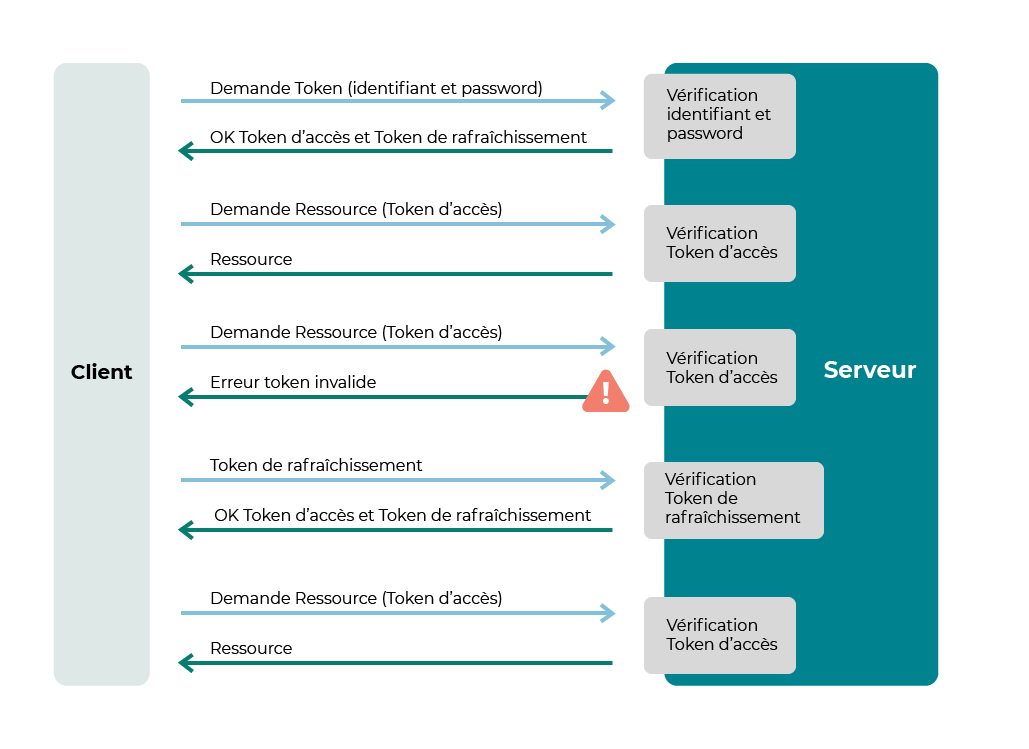
\includegraphics[width=12cm]{images/image23.png}
\end{center}
Le client envoie des demandes pour accéder aux ressources au serveur avec des tokens. Si le token est valide, le serveur envoie la ressource et un token de rafraîchissement.
Le client fournit des tokens au serveur pour accéder aux ressources

\subsection{Obtenez des tokens}
La {\color{monOrange}gestion des tokens} est un processus réalisé par les applications clientes – voyons ensemble comment fonctionne ce processus. Dans ce cours, nous allons utiliser \href{https://www.postman.com}{Postman}. Il s’agit d’un outil permettant de modifier toutes les informations de la requête qui appelle notre API. Dans le cas de {\color{monOrange}l’authentification}, nous aurons besoin entre autres de modifier les headers des requêtes.

Vous pouvez obtenir des tokens via un appel POST sur l'endpoint d’obtention de tokens que nous avons configuré dans le projet.

Un identifiant et un mot de passe doivent être fournis dans le corps de la requête, sous les noms {\tt username}  et {\tt password}. Lorsque l’authentification est en succès, alors une paire de tokens est retournée.
\begin{center}
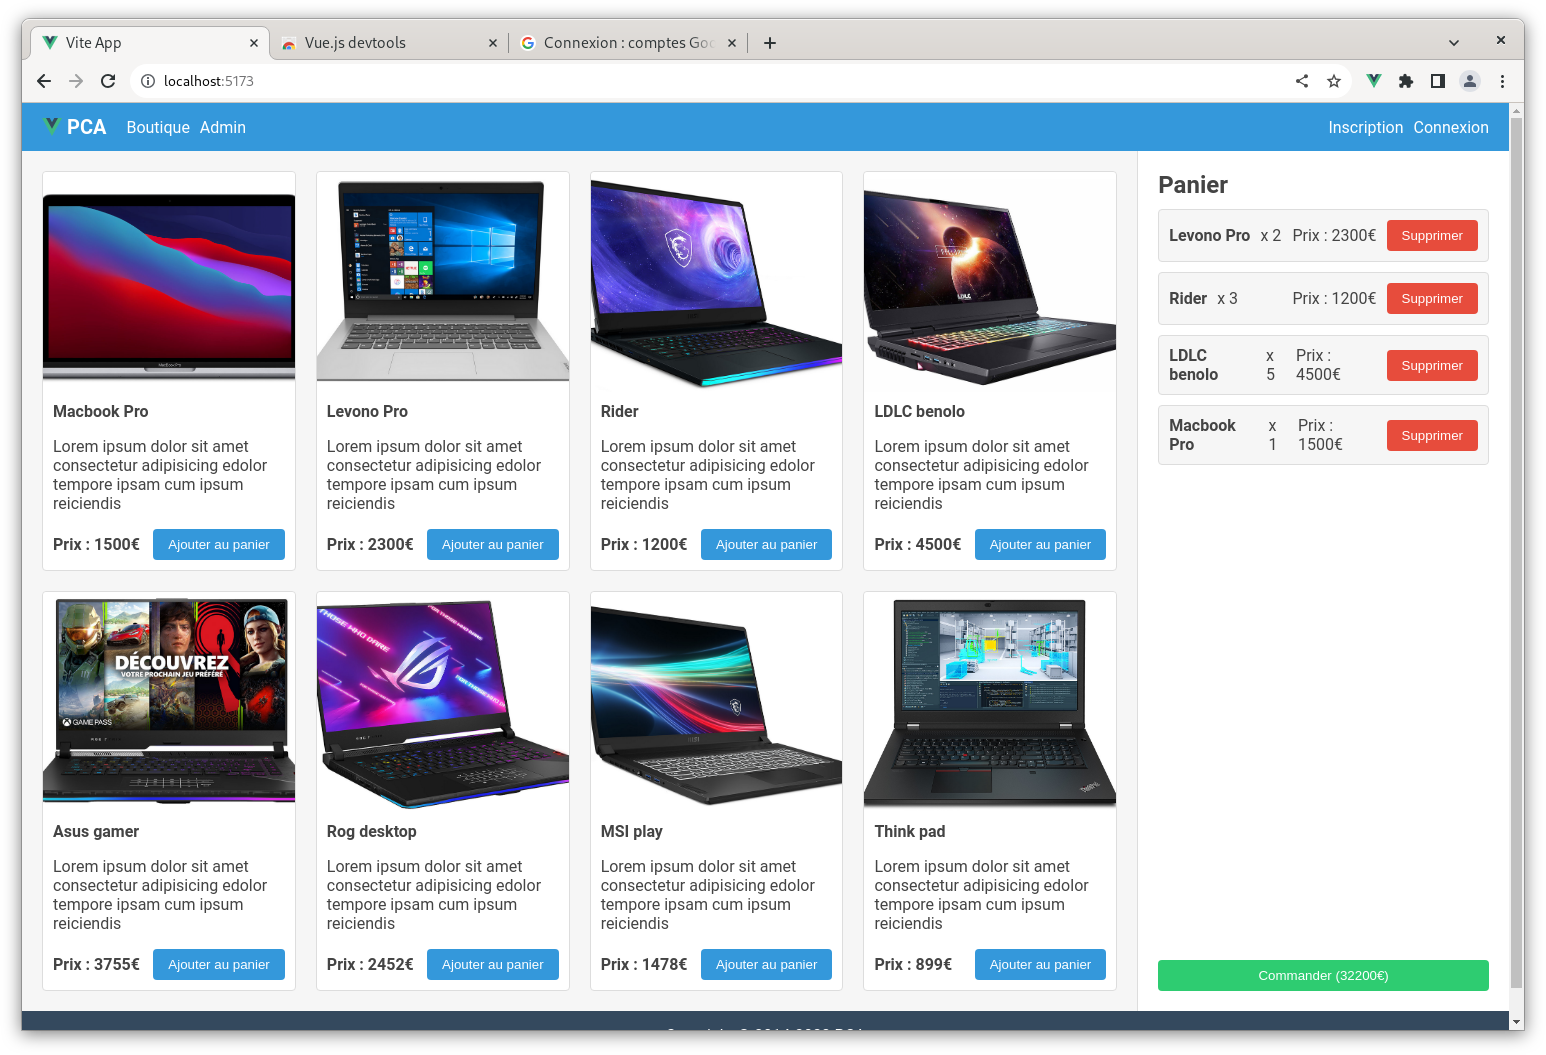
\includegraphics[width=15cm]{images/image24.png}
\end{center}
En entrant l’identifiant admin-oc et le mot de passe password-oc, nous obtenons bien deux tokens refresh et access, une paire de tokens sont retournés

\subsubsection*{C’est quoi Postman ? Pourquoi on ne reste pas dans le navigateur ?}
C’est un outil de gestion de collection d’API très utile lorsqu’on travaille en équipe, mais aussi disponible gratuitement pour un seul utilisateur. Il permet de {\color{monOrange}sauvegarder des appels API} et de réaliser plus facilement le {\color{monOrange}paramétrage de nos appels} (gestion des headers, corps de la requête, etc.).

Nous pouvons voir que chaque token est un JWT, et consiste en 3 parties séparées par des points. Chacun de ces tokens a un {\color{monOrange}rôle bien spécifique} et doit être {\color{monOrange}conservé} par l’application cliente afin de garantir la connexion de l’utilisateur.

Le token d’accès doit être transmis dans le header de chaque requête faite au serveur dans la clé nommée {\tt Authorization}. Cette clé doit avoir pour valeur  {\tt Bearer TOKEN}, en remplaçant  {\tt TOKEN}   par la valeur du token d’accès.



Dans l’onglet Headers, nous voyons la clé Authorization et le Bearer TOKEN associé
La clé Authorization et le Bearer TOKEN
\begin{center}
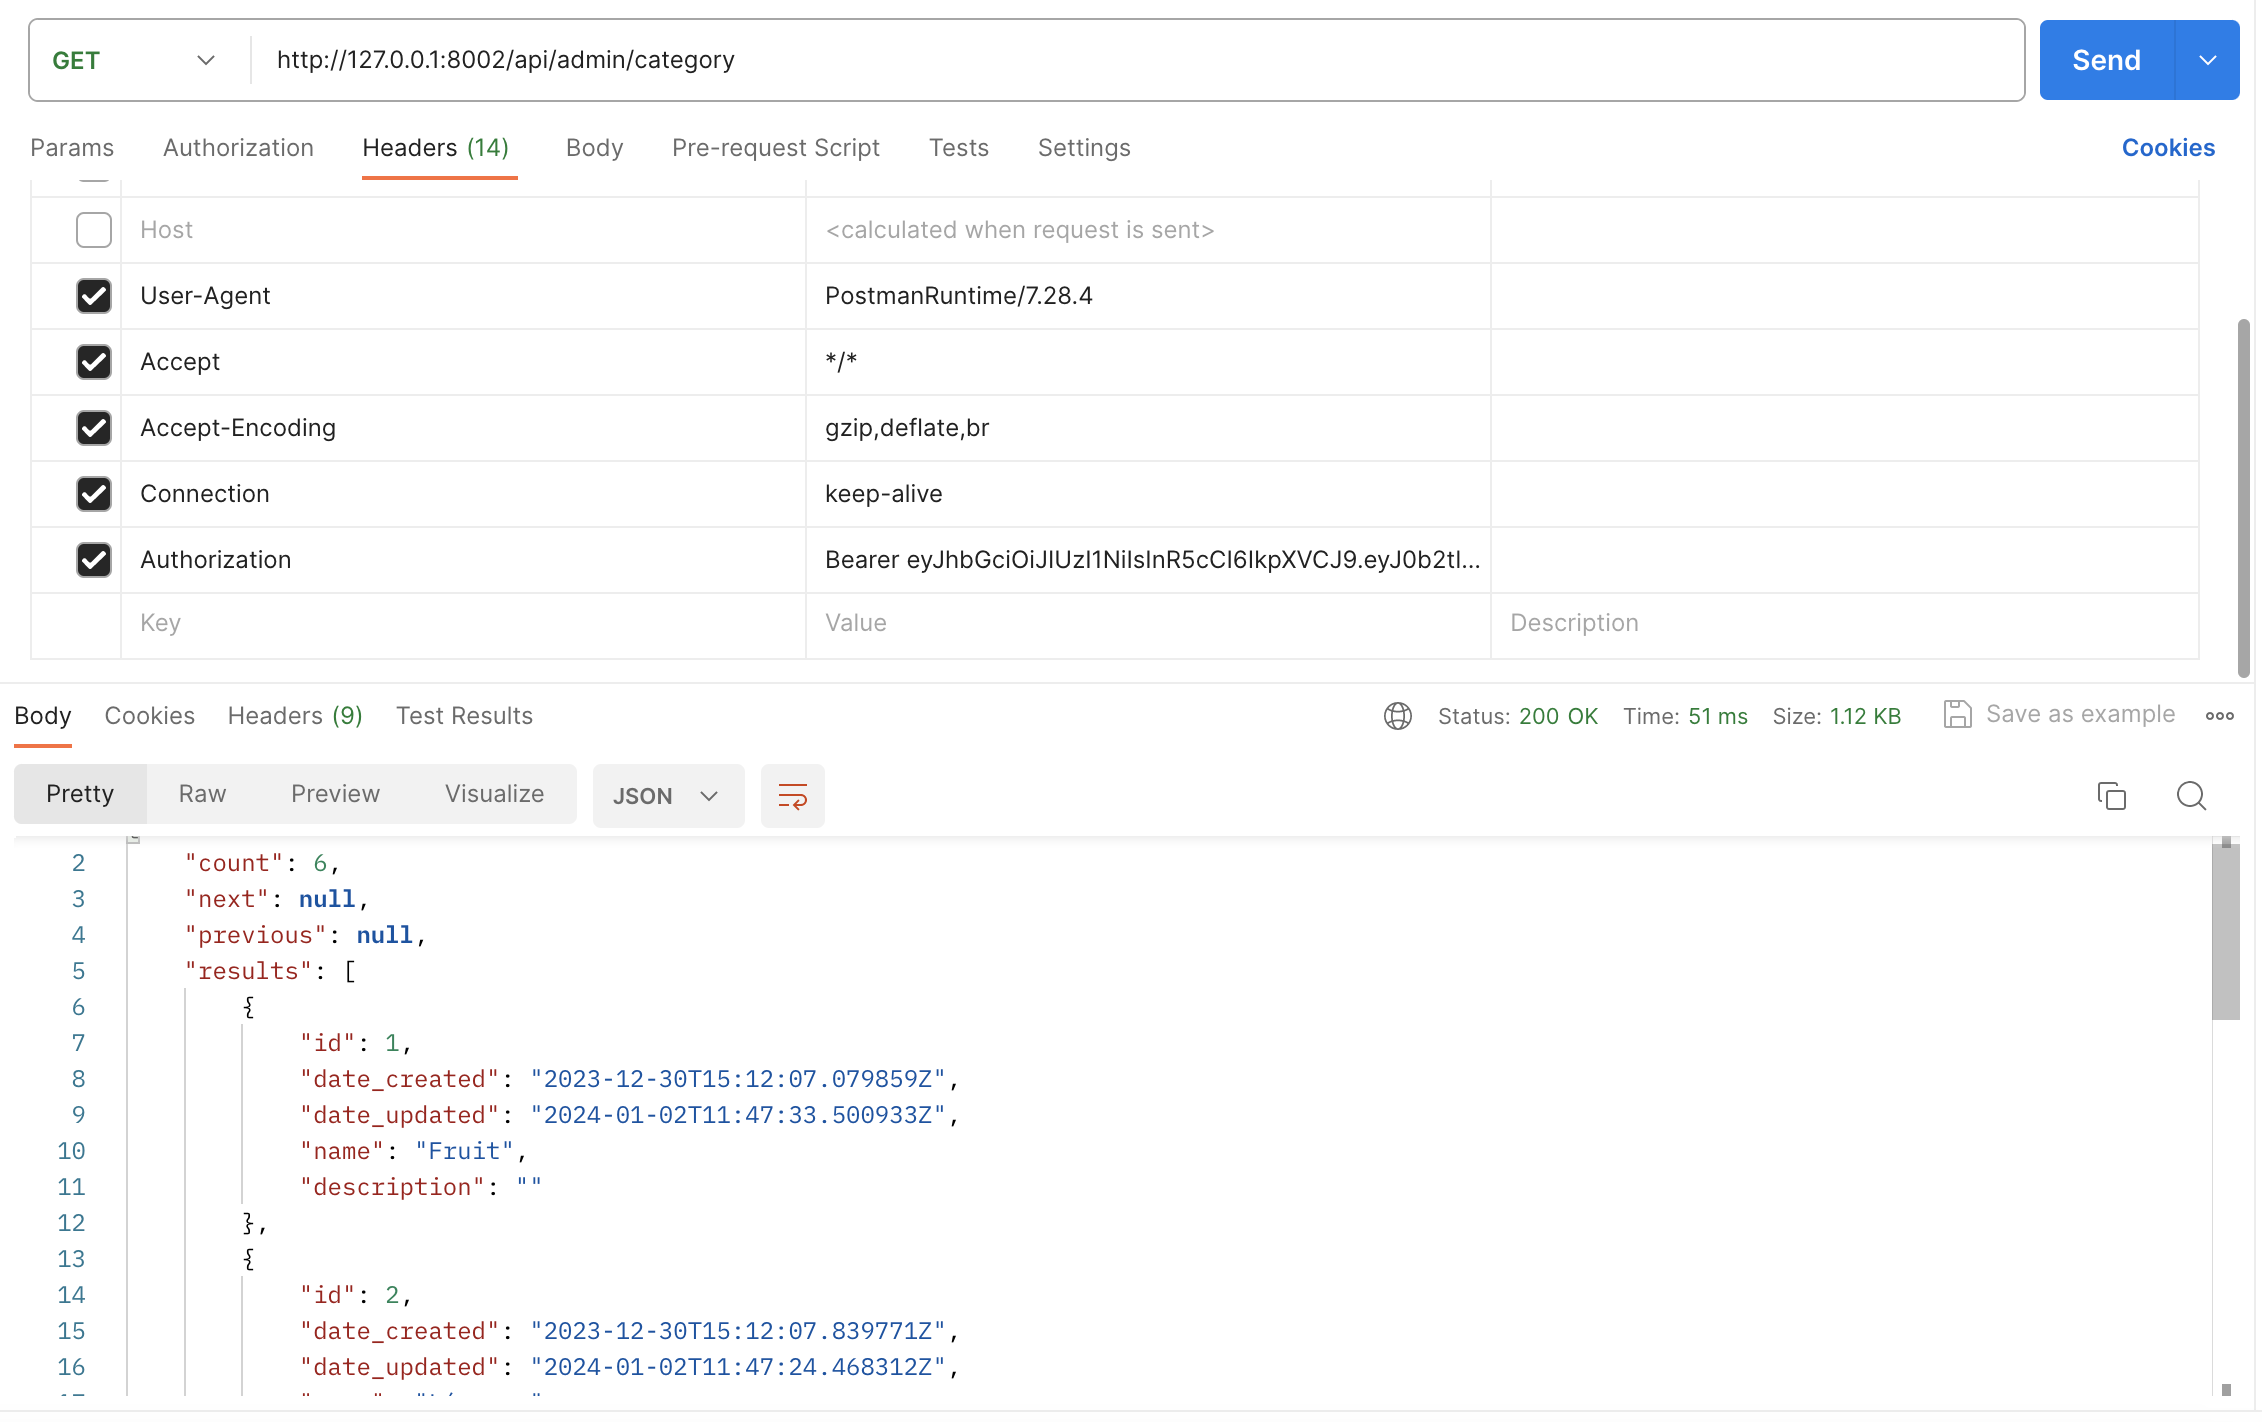
\includegraphics[width=15cm]{images/image25.png}
\end{center}

De cette façon, le serveur, en recevant la requête, peut déterminer l’utilisateur réalisant la requête.

Le token d’accès a une durée de vie {\color{monOrange}limitée dans le temps} ; si nous décodons son payload en utilisant par exemple jwt.io :
\begin{minted}[
mathescape,
framesep=2mm,
baselinestretch=1.2,
%fontsize=\footnotesize,
bgcolor=LightGray,
%linenos
]{python}
{
    "token_type": "access",
    "exp": 1628927720,
    "jti": "63e4e6dab0494aee803fed93f24a80c1",
    "user_id": 1
}
\end{minted}

... nous pouvons voir différentes informations :
\begin{itemize}
\item {\tt token\_type}  indique le type de token ;
\item {\tt exp}  est un timestamp indiquant jusqu’à quand ce token peut être utilisé ;
\item {\tt jti}  signifie JWT ID, c’est un identifiant unique créé lors de la génération du token ;
\item {\tt user\_id}  est l’identifiant Django de l’utilisateur, il est ajouté par Simple JWT lors de la génération du token.
\end{itemize}

\subsubsection*{Est-il possible de modifier la durée de vie des tokens ?}
Oui, la durée de vie des tokens peut être configurée dans les settings de Django.
\begin{minted}[
mathescape,
framesep=2mm,
baselinestretch=1.2,
%fontsize=\footnotesize,
bgcolor=LightGray,
%linenos
]{python}
SIMPLE_JWT = {
    'ACCESS_TOKEN_LIFETIME': timedelta(minutes=5),
    'REFRESH_TOKEN_LIFETIME': timedelta(days=1),
}
\end{minted}

\subsection{Rafraîchissez des tokens}
Lorsque le token d’accès n’est plus valide, il est nécessaire d’en créer un autre. C’est à cela que sert le {\color{monOrange}token de rafraîchissement}.

Il faut pour cela réaliser un appel en POST sur l’endpoint de rafraîchissement de tokens. Le token de rafraîchissement doit être transmis dans le corps de la requête sous l’attribut {\tt refresh}  , et un nouveau token d’accès est alors retourné par le serveur.
\begin{center}
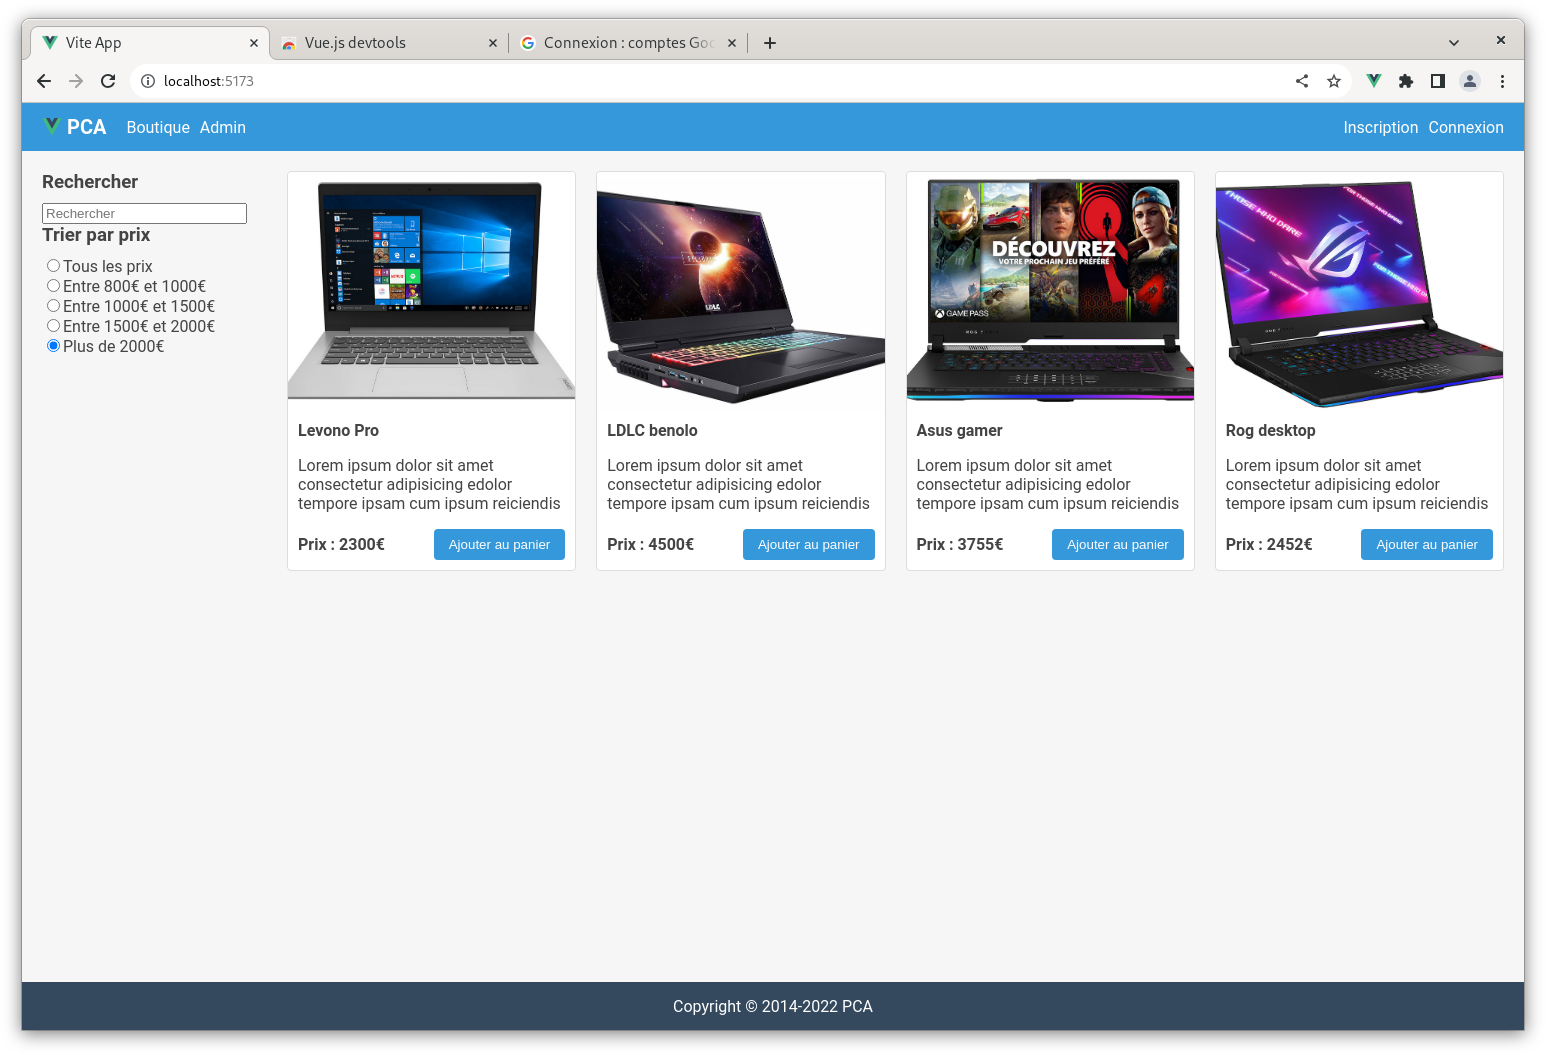
\includegraphics[width=15cm]{images/image26.png}
\end{center}
Quand nous envoyons le token de rafraîchissement, un token d’accès nous est retourné dans Postman
Le token de rafraîchissement permet d’obtenir un nouveau token d’accès
Voyons comment réaliser ces appels ensemble dans le screencast ci-dessous.


N’hésitez pas à tester le fonctionnement des tokens, comment et quand ils expirent. Chaque matin en reprenant le développement du votre projet, vos tokens devront être rafraîchis, c’est signe que l’authentification fonctionne. ;)

Le code du projet est disponible sur la branche P3C1-C2 du projet. Expérimentez la gestion des tokens comme le ferait une application cliente, afin que ce processus n’ait plus de secret pour vous !

\subsubsection*{En résumé}
\begin{enumerate}
\item Les tokens JWT sont un moyen d’assurer l’authentification des utilisateurs.
\item Les tokens d’accès et de rafraîchissement sont à conserver précieusement par les applications clientes pendant la session des utilisateurs.
\item Deux endpoints différents permettent d’une part l’obtention de tokens, et d’autre part le rafraîchissement du token d’accès.
\end{enumerate}

 {\em Maintenant que notre serveur nous permet d’obtenir et de rafraîchir des tokens, voyons dès le prochain chapitre comment limiter l’accès à certains endpoints}.
%%%%%%%%%%%%%%%%%%%%%%%%%%%%%%%%%%%%%%%%%%%%%%%%%%%%%%%%%%%%%%%%%%%%%%%%

\section{Restreignez l'accès à certains endpoints}
\subsection{Limitez l’accès aux utilisateurs authentifiés}
Nous disposons maintenant d’endpoints d’administration qui permettent de gérer pleinement des entités, mais leur accès est pour le moment {\color{monOrange}public}. Améliorons cela en imposant aux utilisateurs d’être authentifiés pour pouvoir faire des appels à nos endpoints d’administration. Commençons par l'endpoint d’{\color{monOrange}administration des catégories}.

DRF nous permet de {\color{monOrange}gérer l’accès aux endpoints} au travers des permissions, et nous propose une permission {\tt IsAuthenticated}, exactement ce qu’il nous faut !

Les permissions se configurent au niveau des views, au travers de l’attribut de classe {\tt permission\_classes}. Cet attribut est une liste, et permet donc d’appliquer plusieurs permissions. Elles sont parcourues une à une par DRF, et l’accès à la vue n’est permis que si toutes les permissions le permettent.

Mettons en place cette permission sur notre {\tt AdminCategoryViewset}  :
\begin{minted}[
mathescape,
framesep=2mm,
baselinestretch=1.2,
%fontsize=\footnotesize,
bgcolor=LightGray,
%linenos
]{python}
from rest_framework.permissions import IsAuthenticated
 
class AdminCategoryViewset(MultipleSerializerMixin, ModelViewSet):
 
    serializer_class = CategoryListSerializer
    detail_serializer_class = CategoryDetailSerializer
    # Nous avons simplement à appliquer la permission sur le viewset
    permission_classes = [IsAuthenticated]
 
    def get_queryset(self):
        return Category.objects.all()
\end{minted}

L’accès à l'endpoint nécessite à présent d’être authentifié en ajoutant dans les headers de la requête POST la clé {\tt Authorization}  qui a pour valeur  {\tt Bearer ACCESS}, où {\tt ACCESS}  est la valeur du token d’accès.

Appel en succès d’un endpoint sécurisé en précisant l’attribut Authorization dans le header de la requête
Appel en succès d’un endpoint sécurisé en précisant l’attribut Authorization dans le header de la requête
\begin{center}
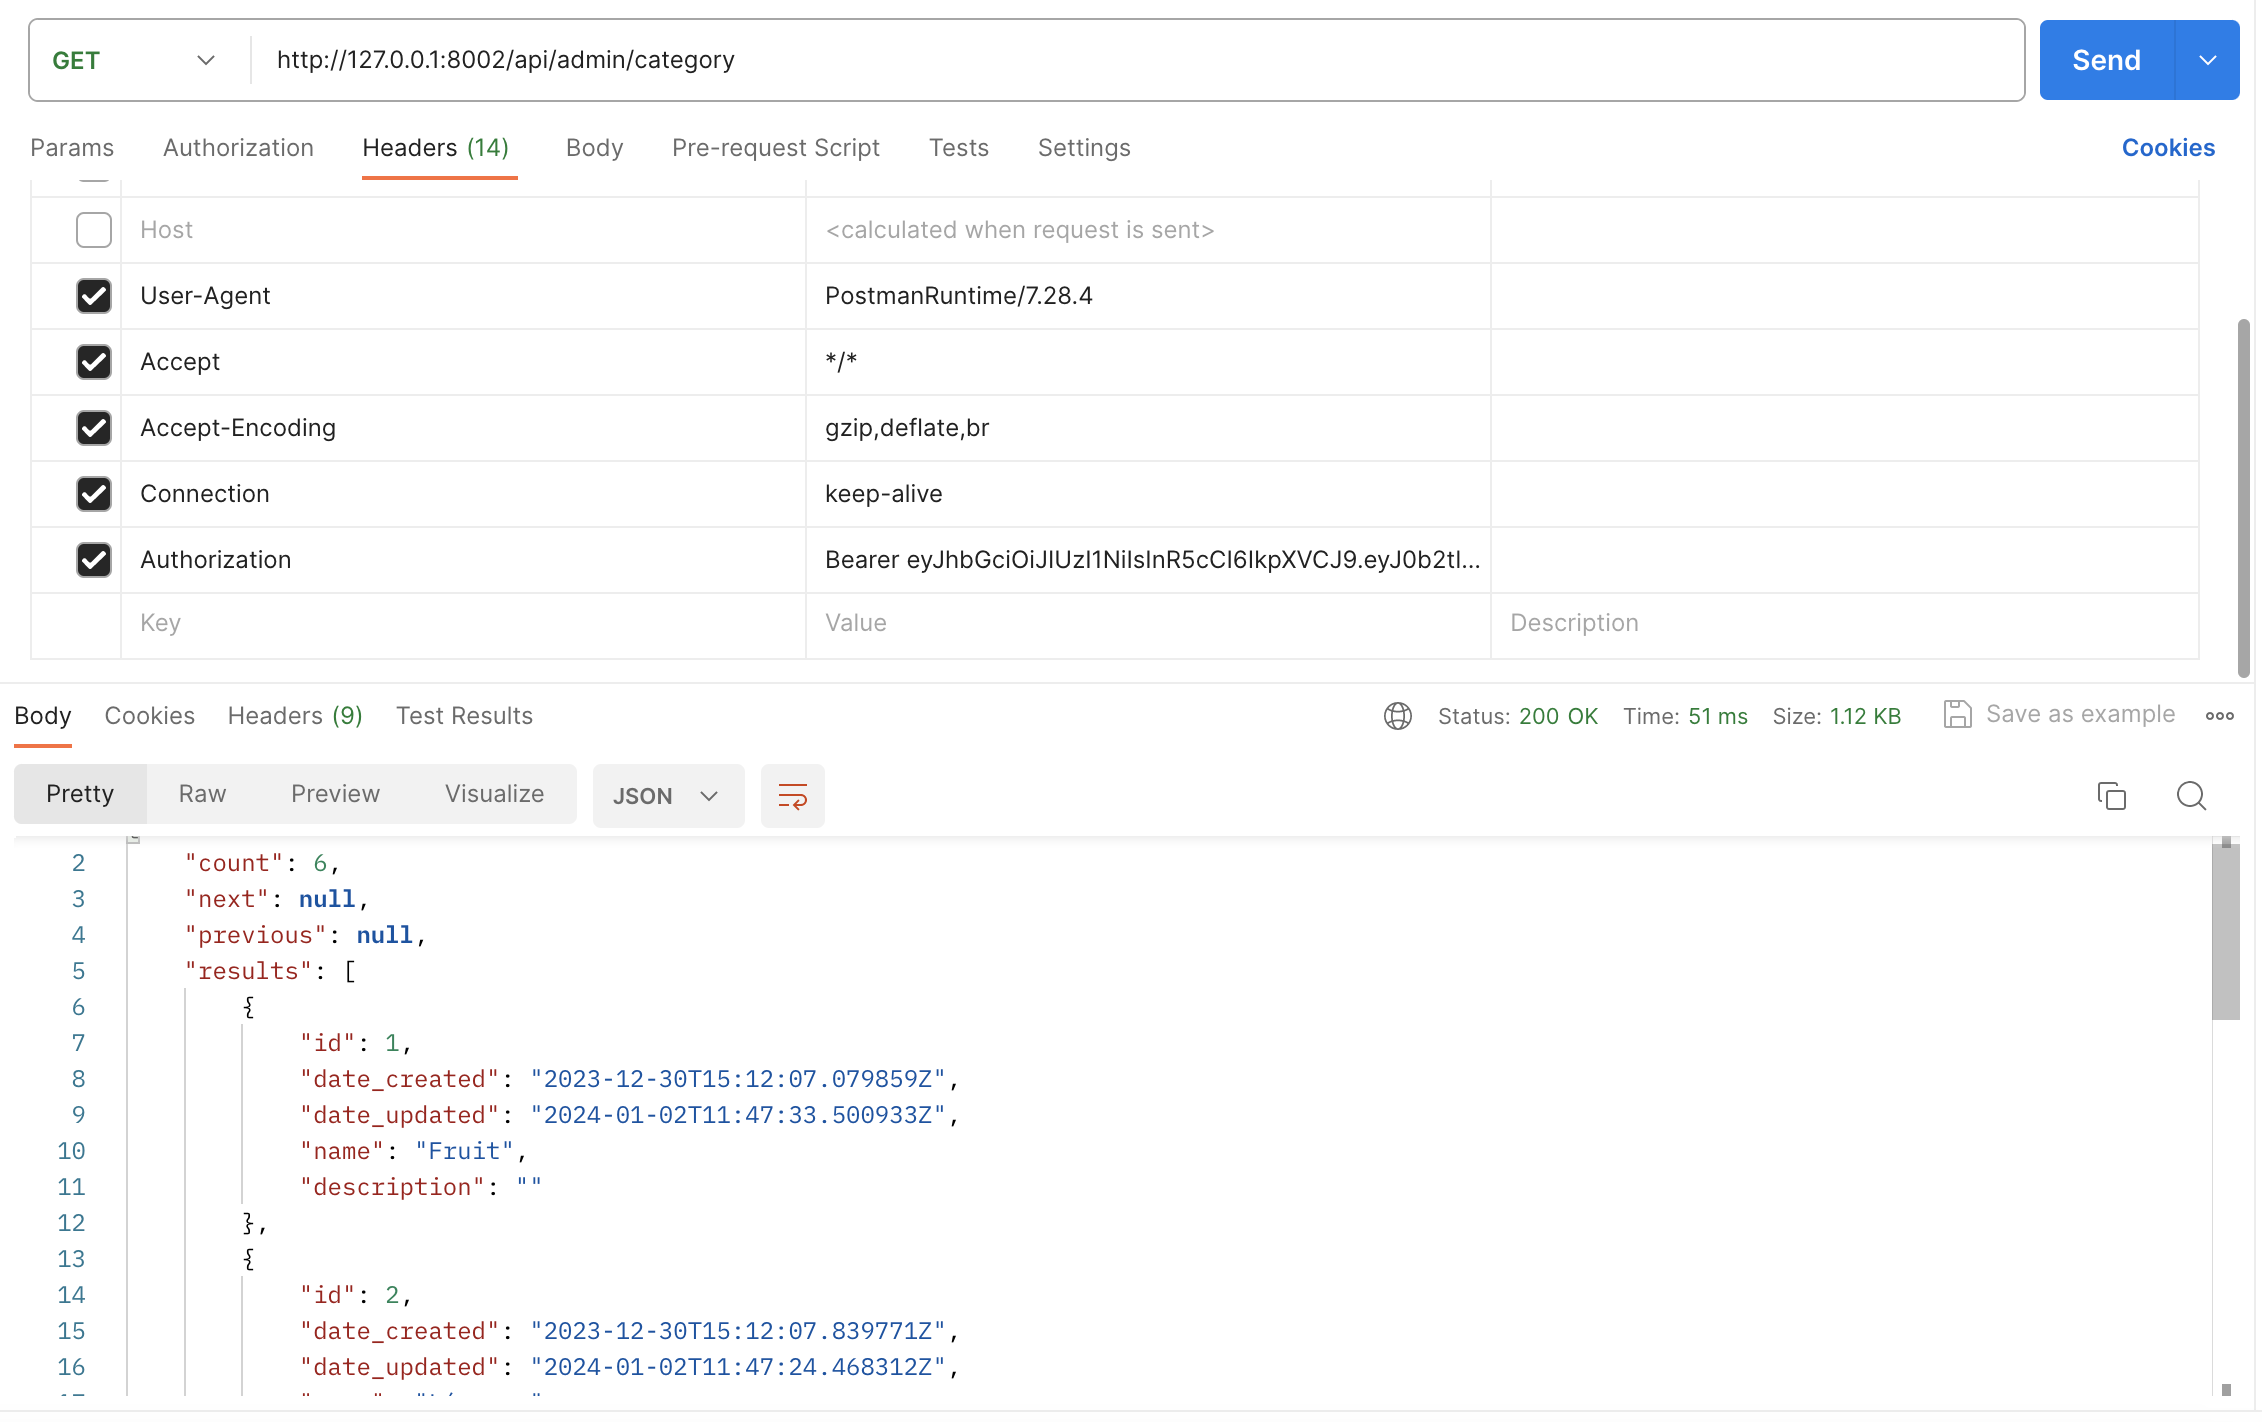
\includegraphics[width=15cm]{images/image25.png}
\end{center}

Vous verrez le status code à droite entre les KEY et la console. Ci-dessus, l'accès a été accepté et un status code 200 est retourné. Sans authentification, un status code 401 est retourné, et l’accès est {\color{monOrange}refusé}.

Un appel sans disposer d’un JWT valide ou sans en fournir sur un endpoint sécurisé retourne un status code 401


Voyons la mise en place d'authentification dans le screencast ci-dessous :

\begin{theorem}
Lors de la création d’un endpoint, il est important de penser à son accès, car il retourne peut-être des informations {\color{monOrange}confidentielles} ou permet des {\color{monOrange}actions} qui ne doivent pas être permises à tout le monde.
\end{theorem}

\subsection{Créez des permissions plus fines}
\subsubsection*{Nous venons de limiter l’accès aux personnes authentifiées, mais est-ce suffisant ?}
La réponse est non, c’est un {\color{monOrange}premier niveau de sécurité}, mais en l’état, les clients de notre boutique pourraient alors administrer nos catégories en disposant seulement d’un compte utilisateur.

DRF propose des permissions, je vous propose encore mieux ! De {\color{monOrange}créer les nôtres}. ;)

Faisons ensemble en sorte que {\color{monOrange}seuls les administrateurs} puissent accéder à cet endpoint. Créons un fichier nommé {\tt permissions.py}  dans notre application Django {\tt shop}.
\begin{minted}[
mathescape,
framesep=2mm,
baselinestretch=1.2,
%fontsize=\footnotesize,
bgcolor=LightGray,
%linenos
]{python}
from rest_framework.permissions import BasePermission
 
class IsAdminAuthenticated(BasePermission):
 
    def has_permission(self, request, view):
    # Ne donnons l’accès qu’aux utilisateurs administrateurs authentifiés
        return bool(request.user and request.user.is_authenticated and request.user.is_superuser)
\end{minted}
Il ne nous reste plus qu’à modifier notre vue pour utiliser notre nouvelle permission :
\begin{minted}[
mathescape,
framesep=2mm,
baselinestretch=1.2,
%fontsize=\footnotesize,
bgcolor=LightGray,
%linenos
]{python}
from shop.permissions import IsAdminAuthenticated
 
class AdminCategoryViewset(MultipleSerializerMixin, ModelViewSet):
 
    serializer_class = CategoryListSerializer
    detail_serializer_class = CategoryDetailSerializer
    permission_classes = [IsAdminAuthenticated]
 
    def get_queryset(self):
        return Category.objects.all()
\end{minted}
Notre endpoint est à présent {\color{monOrange}protégé} et accessible seulement aux {\color{monOrange}administrateurs authentifiés}. Un simple compte utilisateur ne suffit plus pour pouvoir y accéder.

Suivez-moi dans le screencast ci-dessous pour voir comment j'ai mis en place des permissions plus fines pour nos administrateurs :


Les permissions permettent la mise en place de règles de contrôle strictes. Avoir une permission par « acteur » (clients, partenaires, utilisateurs, administrateurs, etc.) de notre API est un bon moyen de gérer qui peut accéder à quels endpoints.

\subsubsection*{Exercice}
Allons plus loin dans nos contrôles ! Pour diverses raisons, un utilisateur administrateur n’est pas membre de l’équipe de la boutique. Il faudrait qu'il puisse n'avoir accès à l’administration qu'en tant que {\color{monOrange}prestataire}, et nous ne souhaitons pas qu’il puisse ajouter de nouvelles catégories.

Je vous propose donc de mettre en place une {\color{monOrange}nouvelle permission} qui va vérifier que l’utilisateur fasse également partie de l’équipe, en vérifiant que {\tt is\_staff}  du model {\tt User}  est bien à {\tt True}.

Les deux permissions pourront alors être mises en place sur le Viewset d’administration de catégorie.

Disposer de deux permissions nous permettra par la suite de donner l’accès à certains endpoints aux membres de l’équipe sans qu’ils aient besoin de disposer d’un compte administrateur, par exemple.

Pour réaliser cela, vous pouvez partir de la branche P2C3\_exercice. Elle contient déjà ce que nous venons de faire ensemble. Une solution est proposée sur la branche P2C3\_solution.

\subsubsection*{En résumé}
\begin{enumerate}
\item Les permissions permettent de limiter l’accès aux endpoints.
\item DRF fournit certaines permissions, mais il est possible de créer les nôtres.
\item Disposer une permission par acteur permet de facilement savoir sur quels endpoints les permissions doivent être placées.
\item Lors de la mise en place d’un nouvel endpoint, il est important de savoir qui va l’utiliser, pour déterminer s’il doit rester public ou doit posséder certaines permissions.
\end{enumerate}
{\em Notre API est toute sécurisée. Je vous invite maintenant à valider vos acquis de cette partie dans le quiz. Après, nous reviendrons sur tout ce que vous avez accompli pendant ce cours !}




\end{document}











    \tableofcontents    

% Fin du document
\end{document}
